
\documentclass[a4paper,12pt,oneside]{book}
\usepackage[utf8]{inputenc}
\usepackage{amssymb}
\usepackage{amsmath}
\usepackage{graphicx}
\usepackage{multirow}
\usepackage{hhline}
\usepackage{caption, subcaption}
\usepackage{graphicx}
\usepackage{mfirstuc}
\graphicspath{Pictures}
\usepackage{geometry}
\usepackage{setspace}
\usepackage{tocloft}
\usepackage{tabu}
\usepackage{fancyhdr}
\geometry{a4paper, tmargin=1in, rmargin=1in, bmargin=1in, lmargin=1.5in}
\usepackage{etoolbox}
\usepackage[svgnames]{xcolor}
\usepackage{comment}
\usepackage{physics}
\usepackage{float}
\usepackage{titletoc}
\usepackage{appendix}
\usepackage{enumitem}
\usepackage{listings}
\usepackage{tikz}
\usepackage{titlesec}
\usepackage{setspace}
\usepackage{indentfirst}
\usepackage{textcase}
\usepackage{pdfpages}
\usepackage[bookmarks, colorlinks=false, pdfborder={0 0 0}]{hyperref}



%-----------------------------------------
% Editables of the document
%-----------------------------------------
\newcommand{\projecttitle}{} % Title of the project, change here

% -----------------------------------------
% STUDENT INFORMATION 
% ------------------------------------------
\newcolumntype{C}[1]{>{\centering}m{#1}}
\newcommand{\studentA}{}
\newcommand{\rollA}{}
\newcommand{\studentB}{}
\newcommand{\rollB}{}
\newcommand{\studentC}{}
\newcommand{\rollC}{}
\newcommand{\guidename}{Mrs. E. Ramalakshmi}
\newcommand{\guidedesignation}{Assistant Professor}
% ---------------------------------------------

% If the number of people is different, change accordingly in titlepage and bonafide certificate
\newcommand{\projectdept}{Information Technology} % Department
 % Project Guide
 % Project Guide
\newcommand{\depthodname}{Dr. M Venu Gopal chari} % Department Head
\newcommand{\depthoddesignation}{Professor and Head, IT} % Department Head
% Also, change the graduation year in titlepage and bonafide certificate
%-----------------------------------------

% References are to be added in reference.bib and cited in any part of the document. Read any examples online on how to add references. You can also use Google Scholar to get the reference formatted for BibTex.


% For Figures and Subfigures


% Package for block commenting


% Chapter and Appendix in TOC prefixed
\makeatletter
\titlecontents{chapter}%
 [0pt]% 
 {\bfseries}%
 {\MakeUppercase \@chapapp\ \thecontentslabel\quad}% 
 {}% 
 {\normalfont\cftdotfill{\cftdotsep}\contentspage}% 
 [\addvspace{0pt}]% 

\g@addto@macro\appendices{%
  \addtocontents{toc}{\protect\renewcommand{\protect\@chapapp}{\appendixname}}%
}
\makeatother


%Package for codes

\lstset{
    breaklines = true,
    captionpos = b,
    numberstyle = \scriptsize,
    numbers=left,                    
    numbersep=10pt
}


% Package for enumerate


% Block Diagram Packages and Functions

\usetikzlibrary{arrows, decorations.markings}
\usetikzlibrary{arrows,positioning,shapes.geometric}
\tikzstyle{vecArrow} = [thick, decoration={markings,mark=at position
   1 with {\arrow[semithick]{open triangle 60}}},
   double distance=1.4pt, shorten >= 5.5pt,
   preaction = {decorate},
   postaction = {draw,line width=1.4pt, white,shorten >= 4.5pt}]
\tikzstyle{innerWhite} = [semithick, white,line width=1.4pt, shorten >= 4.5pt]
\tikzstyle{block} = [draw, fill=blue!20, rectangle, 
    minimum height=3em, minimum width=6em]


\titleformat{\chapter}[display]
{\fontsize{24pt}{24pt}\bfseries\centering}{\MakeUppercase\chaptertitlename\ \thechapter}{5pt}{\ExLarge}
\titlespacing*{\chapter}{}{}{20pt}

% Section Customization
\titleformat{\section}{\fontsize{16pt}{16pt} \bfseries}{\thesection}{1em}{}

% Sub-Section Customization
\titleformat{\subsection}{\fontsize{12pt}{12pt} \bfseries}{\thesubsection}{1em}{}


% Align the titles of auxiliary content to center
\renewcommand*\contentsname{\Large \centerline{Table of Contents}}
\renewcommand*\listfigurename{\Large \centerline{List of Figures}}
\renewcommand*\listtablename{\Large \centerline{List of Tables }}
% \renewcommand*\listabbreviations{\Large \centerline{ABBREVIATIONS}}


% References Addition
\usepackage[backend=bibtex,
style=numeric,
bibencoding=ascii,
maxbibnames=99,
sorting=none
%style=alphabetic
%style=reading
]{biblatex}
\addbibresource{reference.bib}

% Page Style
\pagestyle{fancy}
\cfoot{}
\rhead{}
\lhead{}
\renewcommand{\headrulewidth}{0pt}
\renewcommand{\footrulewidth}{0pt}

\pagestyle{fancy}

%\rhead{}
%\lhead{}

%\renewcommand{\footrulewidth}{0.4pt}

% Line Spacing


%\titleformat{\chapter}[display]{CHAPTER \thechapter}{}{}

%\titleformat{\chapter}
%{\bfseries\centering\Large\filright}{}{}
%%{\Large CHAPTER \thechapter}{\newline}{\Large}
%%\titlespacing*{\chapter}{0pt}{30pt}{20pt}

\titleformat{\section}
{\normalfont\Large\bfseries}
{\thesection}{1em}{}

\titleformat{\subsection}
{\normalfont\large\bfseries}
{\thesubsection}{1em}{}

\titleformat{\subsubsection}
{\normalfont\bfseries}
{\thesubsubsection}{1em}{}

\captionsetup{labelfont=bf}



\begin{document}
\captionsetup{belowskip=0pt}
% To expand the word spacing
\spaceskip=1.5\fontdimen2\font plus 1.5\fontdimen3\font
minus 1.5\fontdimen4\font
\setlength{\textfloatsep}{0.1cm}
\addtolength{\parskip}{-0.5mm}

\frontmatter
\pagenumbering{gobble}
\begin{titlepage}
\begin{center}
\vspace{2cm} 


\normalsize \textbf{A \\[0.075in] Project Report\\ [0.075in]on}  \\
[0.075in]

\Large{\textbf{Edge-Driven CO2 and Occupancy Prediction with Certificate Generation for Optimized Classroom Ventilation Systems}}
\\%\\[0.5in]
\vspace{1.5em}%
\normalsize\textbf{is submitted in partial fulfillment of the Requirements\\ [0.075in]
for the Award of the Degree of} \\ [0.075in]
\vspace{1.5em}
\uppercase{\bf{\textsc{BACHELOR OF ENGINEERING}}} \\
\vspace{0.5em}

in \\
\vspace{0.5em}

\textbf{INFORMATION TECHNOLOGY} \\
\vspace{0.5em}
 Submitted by\\

	\begin{table}[h!]
		\centering
		\begin{tabular}{l l}
			\textbf{Chinthalagari Bhavitha} & \textbf{160121737005}\\ [0.075in]
			
   \textbf{Sri Harsha Goruganti} & \textbf{160121737033}\\ [0.075in]
   \textbf{Vangipuram Sree Raghu Vardhan} & \textbf{160121737061} \\ [0.075in]
			
		\end{tabular} 
	\end{table}

SUPERVISOR\\ [0.075in]
\textbf{Mrs. E. Ramalakshmi }\\ [0.075in]
\textbf{Assistant Professor, IT}\\ [0.075in]


%\begin{figure}[h!]
%	\centering
%	\includegraphics[scale=0.2]{Pictures/logo}
%\end{figure}

\begin{center}
\begin{figure*}[h!]
	\centering
	\includegraphics[scale=0.5]{Pictures/CBIT.png}
	\caption*{\textbf{DEPARTMENT OF INFORMATION TECHNOLOGY}}
	\caption*{\textbf{CHAITANYA BHARATHI INSTITUTE OF TECHNOLOGY(A)}}
	\caption*{\textbf{(Affiliated to Osmania University;Accredited by NBA,NAAC,ISO)}}
	\caption*{\textbf{kokapet(V),GANDIPET(M),HYDERABAD-500075\\}}
\caption*{\textbf{Website:www.cbit.ac.in}}
\end{figure*}


\textbf{2024-2025}
\end{center}

\end{center}
\end{titlepage}
\thispagestyle{empty}
\vspace{3cm}
\begin{center}
%	\textbf{CHAITANYA BHARATHI INSTITUTE OF TECHNOLOGY}\\
%	\textbf{An Autonomous Institute,Affiliated to Osmania University}\\
%	\textbf{Department of Information Technology}\\
	\begin{figure}[h!]
	\centering
	\includegraphics[scale=0.5]{Pictures/logo.png}
	
\end{figure}
	\Large{\textbf{DECLARATION}}
\end{center}

\vspace{0.3cm}

\noindent
\fontsize{12pt}{24pt}\selectfont 

We hereby declare that the project titled \textbf{Edge-Driven CO2 and Occupancy Prediction
with Certificate Generation for Optimized
Classroom Ventilation Systems} is original and has been carried out by us under the supervision of \textbf{Mrs. E. Ramalakshmi }, Associate Professor, Dept. of IT, CBIT, Hyderabad  for the Degree of Bachelor of Engineering in Information Technology, CBIT and the project has been checked using anti-plagiarism software (Turnitin), with a recorded similarity index of 10\%.  If anything found guilty/copied from other sources we are the solely responsible for the same and we abide for any action taken by the Institute authorities. (As per the Institute guidelines, the Supervisor also held responsible for any manipulation by the Student).

% \begin{table}[h!]
% 	\setstretch{1.2}
% 	\centering
% 	\begin{tabular}{l C{2.5cm} l}
% 		\textbf{Place:} && \textbf{Signature:}\\
% 	\textbf{Date:} &&
	
% \end{tabular}
%     \documentclass{article}
% \usepackage{array}
% \usepackage{setspace}
% \usepackage[a4paper, margin=1in]{geometry}
\noindent\textbf{Place: Hyderabad}\\
\textbf{Date:} {\hspace{5cm}}

\begin{flushright} 
\textbf{Student Signatures}\\
\textbf{Chinthalagari Bhavitha }, \textbf{160121737005}\\
\textbf{Sri Harsha Goruganti}, \textbf{160121737033}\\ \textbf{Vangipuram Sree Raghu Vardhan }, \textbf{160121737061}
\end{flushright}


\begin{table}[h!]
    \setstretch{1.2}
    \begin{tabular}{l l l}
        \textbf{Signature of the Supervisor} & & \\
        \textbf{\guidename} & & \\
        \textbf{\guidedesignation, Dept. of IT.} & & \\
        \textbf{CBIT, Hyderabad.}
    \end{tabular}
\end{table}










\newpage
\thispagestyle{fancy}

\begin{center}
\begin{figure}[h!]
	\centering
	\includegraphics[scale=0.5]{Pictures/logo.png}
	
\end{figure}

%	\textbf{CHAITANYA BHARATHI INSTITUTE OF TECHNOLOGY}\\
%	\textbf{An Autonomous Institute,Affiliated to Osmania University}\\
%	\textbf{Department of Information Technology}\\
	\vspace{0.5cm}
	\Large{\textbf{CERTIFICATE}}
\end{center}

\vspace{0.3cm}

\noindent
\fontsize{12pt}{24pt}\selectfont This is to certify that the project work entitled \textbf{Edge-Driven CO2 and Occupancy Prediction with Certificate Generation for Optimized Classroom Ventilation Systems} is submitted by	\textbf{Chinthalagari Bhavitha } \textbf{(160121737-}
 \textbf{005)},
\textbf{Sri Harsha Goruganti} \textbf{(160121737033)}, and
\textbf{Vangipuram Sree Raghu Vardhan} \textbf{(160121737061)}  in partial fulfillment of the requirements for the award of the degree of \textbf{Bachelor of Engineering} in \textbf{\projectdept} to \textbf{CHAITANYA BHARATHI INSTITUTE OF TECHNOLOGY(A)} affiliated to \textbf{OSMANIA UNIVERSITY},Hyderabad is a record of bonafide work carried out by them under my supervision and guidance.The results embodied in this report have not been submitted to any other University or Institute for the award of any other Degree or Diploma.


\vspace{4cm}

\begin{table}[h!]
	\setstretch{1.2}
	\centering
	{\small
	\begin{tabular}{l C{1cm} l}
    \textbf{Signature of the Supervisor}&& \textbf{Signature of the HoD}\\
		\textbf{\guidename} && \textbf{\depthodname}\\
		\textbf{\guidedesignation, Dept. of IT,} & &\textbf{\depthoddesignation,}\\
	\textbf{CBIT, Hyderabad.} & &\textbf{CBIT, Hyderabad.}\\
	\end{tabular}
	}
\end{table}




\renewcommand{\footrulewidth}{0.4pt}
\cfoot{\small{Kokapet(V),Gandipet(M),Ranga Reddy (Dist.)–500075, Hyderabad, T.S.\\
		 www.cbit.ac.in}}



\clearpage
\pagenumbering{roman}
\fontsize{12pt}{12pt}\selectfont
\onehalfspacing
\addtocontents{toc}{\textbf{Title}\hfill\textbf{Page No.}\par}
\fancyfoot{}
\renewcommand{\footrulewidth}{0pt}
\input{acknowledgements.tex}
\clearpage
\phantomsection
\addcontentsline{toc}{chapter}{Abstract}
\chapter*{Abstract}
As indoor air quality (IAQ) becomes increasingly critical in educational settings, optimizing classroom ventilation systems is essential for enhancing student and teacher well-being. This study presents an innovative edge computing-based approach that combines IoT sensors, LSTM neural networks, and cloud integration to create an intelligent ventilation management system. By deploying low-cost IoT devices equipped with environmental sensors and edge computing capabilities, our solution collects and processes data at the classroom level. A lightweight LSTM model implemented on edge devices provides real-time predictions of ventilation quality and occupancy patterns, enabling immediate environmental adjustments. The system architecture features a hierarchical design that includes local edge devices for data acquisition and initial predictions, an intermediate fog layer utilizing Raspberry Pi for aggregation and building-wide decision-making, and cloud services (ThingSpeak) for long-term data storage and analysis. The real-time data processing with minimal latency, and comprehensive environmental quality certificates. The system successfully monitors and analyzes key parameters including temperature, humidity, CO2 levels, and occupancy rates, demonstrating its effectiveness in maintaining optimal classroom conditions. The integration of edge computing with machine learning and IoT technologies delivers improved precision in environmental quality evaluation, making it highly useful for educational institutions.
\\
\\

\textbf{\textit{Keywords}}:
Smart Classroom, Environmental Quality, CO\textsubscript{2}
 Prediction, LSTM, Edge Computing, Occupancy Monitoring, Ventilation Control, Certificate Generation


\clearpage
\phantomsection
%\addcontentsline{toc}{chapter}{Table of Contents}
\tableofcontents

% List of Figures Page
\clearpage
\phantomsection
\addcontentsline{toc}{chapter}{List of Figures}
\listoffigures

% List of Abbreviations Page
\clearpage
\phantomsection
\addcontentsline{toc}{chapter}{Abbreviations}
\newlist{abbrv}{itemize}{1}
\setlist[abbrv,1]{label=,labelwidth=1in,align=parleft,itemsep=0.1\baselineskip,leftmargin=!}

\begin{center}
\textbf{\large{Abbreviations}}
\end{center}
\vspace{1cm}
\begin{abbrv}
  \item[\textbf{Abbreviation}] \hspace{2.25cm}\textbf{Description}
  \item[AI] \hspace{2cm} Artificial Intelligence
  \item[AMP] \hspace{2cm} Automatic Mixed Precision
  \item[API] \hspace{2cm} Application Programming Interface
  \item[CO₂] \hspace{2cm} Carbon Dioxide
  \item[DHT11] \hspace{2cm} Digital Humidity and Temperature Sensor
  \item[GPIO] \hspace{2cm} General Purpose Input/Output
  \item[HVAC] \hspace{2cm} Heating, Ventilation, and Air Conditioning
  \item[IoT] \hspace{2cm} Internet of Things
  \item[KPIv] \hspace{2cm} Key Performance Indicator for Ventilation
  \item[LCD] \hspace{2cm} Liquid Crystal Display
  \item[LSTM] \hspace{2cm} Long Short-Term Memory
  \item[PM2.5] \hspace{2cm} Particulate Matter ≤ 2.5 Microns
  \item[RAM] \hspace{2cm} Random Access Memory
  \item[RNN] \hspace{2cm} Recurrent Neural Network
  \item[RPi] \hspace{2cm} Raspberry Pi
  \item[RTOS] \hspace{2cm} Real-Time Operating System
  \item[UART] \hspace{2cm} Universal Asynchronous Receiver-Transmitter
  \item[VOC] \hspace{2cm} Volatile Organic Compound
\end{abbrv}


\newcommand*\subtxt[1]{_{\textnormal{#1}}}
\DeclareRobustCommand\_{\ifmmode\expandafter\subtxt\else\textunderscore\fi}

\newcommand*\suptxt[1]{^{\textnormal{#1}}}
\DeclareRobustCommand\^{\ifmmode\expandafter\suptxt\else\textunderscore\fi}

% Main Content
\mainmatter
\rfoot{\thepage}
\rhead{}
%\rhead{\textbf{\projecttitle}}
\lhead{}
\lfoot{\small{Department of Information Technology}}
%\renewcommand{\headrulewidth}{0.4pt}
\renewcommand{\footrulewidth}{0.4pt}
\setstretch{1.5}
\chapter{Introduction}

\section{Origin of Proposal}
Indoor air quality significantly impacts cognitive ability, comfort, and overall health, especially in tightly occupied areas such as classrooms. Traditionally, indoor ventilation management has relied on static, threshold-based systems or manual operations that lack responsiveness to real-time environmental changes. These approaches are often inefficient, unable to account for varying occupancy levels or fluctuating CO\textsubscript{2} concentrations, and offer limited adaptability in dynamic learning environments.Existing monitoring systems fail to integrate predictive modeling with localized control, leading to inconsistent ventilation performance and energy inefficiencies. The challenge lies in developing a responsive system capable of collecting real-time data, interpreting temporal patterns, and adjusting ventilation intelligently. Advancements in edge computing and deep learning, particularly through Long Short-Term Memory (LSTM) networks, provide new opportunities for accurate forecasting of indoor conditions.

This proposal arises from the need for a robust, predictive, and automated classroom ventilation solution. It seeks to ensure healthy air quality, sustainable energy usage, and real-time certification of environmental standards, contributing to smarter and healthier educational infrastructure.

\section{Definition of Problem}
Accurate prediction and control of indoor CO\textsubscript{2}   levels in educational spaces are vital for improving cognitive performance, maintaining occupant comfort, and ensuring a healthy learning environment. However, several challenges hinder effective ventilation optimization. Environmental data from classrooms often display fluctuations due to changing occupancy levels, variable room sizes, and diverse usage patterns, complicating the task of consistent air quality regulation. Additionally, the latency and limitations of cloud-based systems in handling real-time control reduce their practicality in fast-changing indoor environments. Edge devices, while beneficial for localized processing, often face resource constraints when dealing with continuous data streams and advanced predictive models. Furthermore, the nonlinear and temporal nature of CO₂ progression demands models that can learn from sequential dependencies rather than static thresholds. Traditional rule-based or shallow learning approaches struggle to capture these complex dynamics. To overcome these limitations, our system integrates a lightweight Long Short-Term Memory (LSTM) model with sensor networks and actuator control, all deployed on edge platforms. This architecture enables timely, adaptive ventilation management with minimal computational overhead while enhancing responsiveness and prediction accuracy across diverse classroom conditions.

\\ 

\section{Objective}
The primary objective of this project is to design, implement, and evaluate a predictive system for real-time classroom air quality management. The goal is to enhance the efficiency, comfort, and sustainability of indoor environments by using machine learning techniques and edge computing to predict air quality and optimize ventilation control. The specific goals are elaborated below:

To develop predictive models using Long Short-Term Memory (LSTM) networks and regression algorithms for accurate CO₂ level forecasting. This project proposes an approach that combines LSTM's ability to capture temporal dependencies in environmental data with regression techniques to refine ventilation control. The motivation behind this design is to forecast future air quality trends, enabling the system to proactively adjust ventilation instead of reacting to changes. The model is expected to improve air quality prediction and ventilation control, adapting to various classroom conditions. To validate its effectiveness, the LSTM-based model will be compared to traditional threshold-based methods and other machine learning approaches.

To implement a real-time data acquisition and monitoring system using low-cost IoT sensors and edge devices. The system will integrate environmental sensors for CO₂, temperature, humidity, and occupancy, all connected to platforms like Raspberry Pi and Arduino. This architecture allows for efficient, low-latency data processing, ensuring real-time air quality assessment while minimizing dependence on cloud infrastructure. The edge-based setup enhances data privacy, speeds up response times, and offers scalability for deployment in multiple classrooms or institutions.

To investigate the influence of key environmental variables on air quality and occupancy patterns within classrooms. This research will identify which factors—such as CO₂ concentration, temperature, and occupancy—affect indoor air quality the most. By recognizing these patterns, the system can better adjust ventilation strategies to improve air quality, ensuring a comfortable learning environment. This will lead to optimized ventilation systems and more effective classroom management, promoting student and faculty health.

To create a decision support tool that recommends the best classroom based on real-time environmental conditions. This tool will assess classroom environments in real time and suggest the optimal room with the best air quality for students and faculty. By doing so, it will help in selecting classrooms that meet air quality standards, ultimately improving learning conditions.

To integrate the predictive air quality system with classroom management tools and cloud platforms for seamless monitoring and data processing. This integration will enable automated air quality tracking, real-time data access, and long-term monitoring, contributing to the development of smarter, healthier classroom environments and supporting the growth of sustainable educational infrastructure.
\newpage
\section{Organization Of the Project}\\
Chapter 1: This introductory chapter provides background information on the importance of classroom air quality and the need for an intelligent ventilation system. It discusses the project's goals, the integration of machine learning for air quality prediction, and the benefits of real-time monitoring in educational environments.

Chapter 2: This chapter reviews existing methods for air quality management and smart classroom systems, with a focus on the use of predictive models like LSTM for environmental forecasting. It also discusses IoT-based data acquisition systems and their role in improving classroom air quality and comfort.

Chapter 3: This chapter outlines the system requirements, both functional and non-functional, for implementing the air quality management system. It details the hardware and software components necessary to deploy the predictive model and the real-time monitoring system.

Chapter 4: The data collection and preprocessing methods used in this project are discussed in this chapter, along with the structure of the predictive model. It describes how environmental sensor data is gathered and how the LSTM model is applied to predict CO₂ levels and inform ventilation control decisions.

Chapter 5: This chapter covers the implementation of the methods, including data handling, model training, and performance evaluation. It discusses the evaluation metrics used, such as accuracy, CO₂ level prediction error, and system responsiveness. A comparative analysis of the model's performance is also presented.

Chapter 6: This chapter presents the findings of the study, highlighting the effectiveness of the predictive model and its impact on air quality management. It also discusses the practical applications of the system for real-time classroom air quality control.

Chapter 7: The final chapter explores potential future enhancements, including advanced data augmentation techniques, real-time adaptation to classroom conditions for large-scale deployment in educational institutions.
\clearpage
\chapter{Literature Survey}

\section{Related Work}  
The growing concern over indoor air quality (IAQ) and energy efficiency has led to extensive research into smart ventilation systems using Internet of Things (IoT) technologies. Early solutions primarily utilized simple sensors with rule-based actuation, which lacked adaptability and real-time optimization. However, the integration of IoT and edge computing has enabled real-time sensing, data-driven control, and intelligent decision-making in ventilation systems. Researchers have developed systems that not only monitor pollutants like CO₂ and PM2.5 but also predict future air quality trends using machine learning models. Studies such as Luo et al. \cite{1} and Rastogi et al.\cite{2} have explored natural ventilation and adaptive ventilation control through IoT-based sensor data. Additionally, embedded systems like those proposed by Mahbub et al. \cite{3} have enabled multifunctional monitoring — including ventilation, lighting, and fire detection highlighting the potential of integrated smart building technologies.

\section{Current State of the Field}  
Contemporary smart ventilation systems utilize embedded platforms (such as ESP32 or Arduino) connected to multi-sensor modules (e.g., MQ-135, DHT11) to continuously monitor air quality indicators. These systems are often linked to cloud or edge-based platforms for real-time control and data visualization. As seen in Tagliabue et al.\cite{4} and Wang et al. \cite{5}, data-driven models such as LSTM and hybrid learning architectures are being used to predict pollutant levels and dynamically adjust ventilation systems. There is also a shift toward deploying models at the edge to reduce latency and dependence on centralized infrastructure. Smart dashboards, cloud APIs, and mobile applications facilitate user interaction and enhance usability. Despite technological progress, challenges such as sensor drift, environmental variability, and energy management still require robust solutions
\section{Recent Developments, Breakthroughs, and Trends}  
Recent advancements in smart ventilation systems research have focused on several key areas. One major development is the integration of edge AI, where machine learning models are deployed directly on edge devices for fast, localized decision-making. This approach enhances system responsiveness, allowing for real-time adjustments in ventilation. Another important direction is the development of multi-room and distributed systems, which optimize air quality across multiple indoor zones simultaneously. These systems enable more coordinated control of indoor environments, improving overall air quality management. Additionally, energy-aware ventilation systems have gained attention, with research emphasizing the balance between energy optimization and air quality enhancement. These systems are aligned with sustainable building goals, focusing on reducing energy consumption while maintaining indoor comfort. Furthermore, data-driven prediction models, particularly Long Short-Term Memory (LSTM) networks and hybrid methods, have been increasingly used for long-term prediction of air quality parameters. These models offer more accurate forecasting capabilities, enhancing the efficiency of ventilation systems. Lastly, low-cost modular IoT platforms have become a significant area of focus, enabling scalable and cost-efficient indoor air quality (IAQ) systems. This trend makes it feasible to implement smart ventilation technologies in various settings, including residential and commercial spaces, thus promoting broader adoption of sustainable indoor air quality management systems.

\section{Key Papers, Researchers, and Organizations}  

\subsection{Key Papers}  
Several influential papers have contributed significantly to the advancement of ventilation systems and IoT-based environmental monitoring. Maohui Luo et al. (2021) demonstrated the use of real-time sensor data to assess the ventilation potential in dynamic environments, highlighting the importance of IoT-based air quality sensors for efficient building ventilation \cite{1}. Rastogi et al. (2021) proposed a context-aware ventilation control system that adapts to indoor environmental parameters, ensuring optimized air quality and energy efficiency \cite{2}. Mahbub et al. (2021) introduced a multi-functional embedded system for indoor ventilation and fire detection, showcasing the integration of IoT in environmental monitoring and safety \cite{3}. Tagliabue et al. (2021) presented an advanced data-driven model for indoor air quality prediction in educational facilities, utilizing a sensor network to enhance IAQ management \cite{4}. Yang et al. (2021) developed a hybrid learning model, BO–EMD–LSTM, for reliable long-term CO₂ concentration forecasting, contributing to accurate predictions for ventilation needs \cite{6}. McNeill et al. (2022) explored IAQ optimization strategies in schools and universities, focusing on real-world applications of room-level ventilation control \cite{7}. Zivelonghi (2023) proposed a smart framework for dynamic, room-specific ventilation control, using IoT to improve air quality across multiple zones in educational environments \cite{11}. Benammar et al. (2018) introduced a low-cost, scalable modular IoT platform for real-time IAQ monitoring, making it feasible to deploy such systems in a variety of indoor settings \cite{16}. El-Sayed et al. (2017) highlighted the integration of edge computing with IoT and cloud technologies for smart environments, emphasizing the role of distributed computing in improving ventilation system performance \cite{14}.




\subsection{Prominent Researchers}  
Several researchers have made notable contributions to the development of IoT-based indoor air quality monitoring and smart ventilation systems. Maohui Luo is widely recognized for his pioneering work in assessing the potential for natural ventilation in buildings using real-time sensor data. His research demonstrated how IoT-based sensor networks can optimize ventilation in dynamic indoor environments, improving both air quality and energy efficiency in diverse building types. K. Rastogi has significantly advanced the field by developing context-aware systems that monitor and control ventilation rates based on changing indoor conditions. His work on adaptive ventilation control using IoT systems has allowed for more efficient management of indoor air quality, which is crucial in maintaining healthy environments in homes, offices, and public spaces. Mobasshir Mahbub’s contributions include the development of cloud-enabled, embedded IoT systems that integrate ventilation control with fire detection and lighting management. His research highlights the importance of multifunctional systems that offer a comprehensive approach to environmental monitoring while improving safety and comfort in indoor spaces. Lavinia Chiara Tagliabue’s work has focused on data-driven approaches to IAQ prediction, particularly in educational settings. She introduced advanced prediction models based on sensor networks to forecast air quality in classrooms, ensuring that ventilation systems could be optimized to enhance comfort and learning conditions. Guangfei Yang’s innovative approach involved hybrid machine learning models, such as BO-EMD-LSTM, for predicting long-term CO₂ concentrations in indoor spaces. His research has enabled more accurate long-term forecasting of air quality, which is essential for maintaining optimal conditions in classrooms and other indoor environments. V. Faye McNeill has worked extensively on optimizing room-level ventilation in schools and universities. Her research focuses on strategies that can improve air quality in individual rooms, offering practical solutions for improving IAQ in real-world academic institutions. Zivelonghi Giuseppi has also made significant strides in dynamic, room-specific air quality control, developing IoT-enabled frameworks that enable real-time air quality optimization across multiple rooms in schools. Mohieddine Benammar contributed to the development of modular IoT platforms for real-time indoor air quality monitoring, providing scalable solutions that can be deployed across various building types. Finally, Hesham El-Sayed’s research in integrating edge computing with IoT and cloud systems has transformed smart ventilation systems by enabling faster processing and real-time decision-making, reducing latency and improving system responsiveness.


\section{Literature Review}  
Recently, a variety of research efforts have focused on exploring advancements in IoT-driven ventilation systems designed to improve indoor air quality, safety, and energy conservation. With the advent of IoT-enabled sensor networks and data-driven frameworks, real-time indoor air quality monitoring and management have become achievable, laying the groundwork for more intelligent ventilation solutions. This survey reviews existing literature on IoT-based ventilation technologies, focusing on sensor innovations, data collection methodologies, machine learning applications, and control strategies that optimize both air quality and energy use.

Luo et al. (2018-2019) explored the potential of natural ventilation (NV) in buildings by deploying IoT-driven environmental sensors in a Berkeley building to monitor indoor air quality, climate, and occupant behavior over a year-long period. Their research showed that NV had the potential to be utilized for 61.2\% of the year, but its actual use was significantly lower, under 35\%. This discrepancy was largely attributed to occupants' preferences, which were not always aligned with the optimal environmental conditions. Occupants often preferred mechanical ventilation or had individual preferences that did not always match the ideal energy-saving strategies provided by natural ventilation. The study suggests that predictive models, which dynamically adjust ventilation strategies based on real-time environmental conditions and occupant behavior, could bridge this gap. Moreover, Luo et al. emphasized the importance of raising user awareness and leveraging advanced predictive models, which could lead to a more widespread adoption of NV, ensuring both improved indoor air quality and energy efficiency \cite{1}.

Rastogi et al. proposed a context-aware IoT-based system for monitoring indoor ventilation by integrating environmental sensors that track key pollutants, such as PM2.5, PM10, CO, and CO2, to detect and mitigate poor ventilation. The system analyzes data through the k-Nearest Neighbors (k-NN) algorithm and achieved impressive results with a precision of 0.91 and an F1-score of 0.89, showcasing its capability in accurately detecting inadequate ventilation. This high level of accuracy allows the system to issue real-time alerts through a smartphone app, enabling immediate corrective actions to enhance air quality. The study demonstrates the effectiveness of data-driven approaches in improving ventilation control, and Rastogi et al. proposed incorporating additional environmental parameters such as light, sound, and occupancy into the system. This would enhance the adaptability and accuracy of the system, making it more effective across various environments with different air quality challenges \cite{2}.

Mobasshir Mahbub et al. developed an automated system for controlling air conditioning and lighting based on occupancy sensors, alongside monitoring other environmental factors like temperature, humidity, CO2, and smoke. The system ensures proper ventilation and fire safety while optimizing energy usage. It allows for remote monitoring and control via mobile phones or computers, offering a robust solution for real-time management of indoor air quality. By storing data in a cloud database, the system provides convenient access for users to monitor conditions remotely. The authors also discussed potential future improvements, such as integrating machine learning for predictive fire detection and enhancing cloud-based visualizations to facilitate deployment in industrial environments or densely populated areas. The ability to integrate smart technologies into existing building management systems could lead to significant advances in indoor air quality management and safety in various settings \cite{3}.

Tagliabue et al. proposed an IoT-based system that integrates indoor air quality (IAQ) data with HVAC (Heating, Ventilation, and Air Conditioning) control systems, aiming to enhance user comfort and performance in educational environments. The system collects real-time data on CO2 levels, temperature, and humidity, forecasting comfort conditions and adjusting ventilation rates using artificial neural networks (ANNs) and Markov predictive models. The results from their system showed reliable predictions, with CO2 forecasts achieving a mean squared error (MSE) of 10.6\%, proving its potential to adjust ventilation dynamically to optimize comfort and air quality. Future work could refine the system by integrating additional parameters, such as occupancy counts, room activity, and user feedback, to improve prediction accuracy and overall system performance. The incorporation of real-time data from users would also enhance the personalization of air quality management in educational settings, benefiting both students and staff \cite{4}.

Wang et al. introduced a novel CT-LSTM (Convolutional Transformer Long Short-Term Memory) model for predicting Air Quality Index (AQI) levels, using both air quality and meteorological data to improve prediction accuracy. By leveraging the powerful capabilities of LSTM networks, the model captures sequential dependencies in air quality data, outperforming traditional predictive models like Support Vector Regression (SVR), Multi-Layer Perceptron (MLP), and basic Recurrent Neural Networks (RNNs). Their model demonstrated superior prediction accuracy, suggesting its applicability to other time-series forecasting problems such as stock market trends and commodity pricing. Wang et al. noted that their model's ability to predict AQI could be a critical tool in public health and environmental monitoring. Future research could focus on enhancing the model with multi-scale spatial predictions, allowing for improved accuracy and broader applicability in various geographical environments \cite{5}.

Yang et al. developed a hybrid BO–EMD–LSTM (Bayesian Optimization-Empirical Mode Decomposition-Long Short-Term Memory) method for predicting indoor CO2 levels, a significant factor in indoor air quality management. This method combines signal decomposition with deep learning and Bayesian optimization techniques, achieving more than 55\% higher accuracy than traditional models, with an R² value exceeding 95\%, which indicates excellent prediction stability. Yang et al. emphasized the speed and high accuracy of the model, making it ideal for real-time applications such as indoor air quality monitoring systems. The use of such advanced techniques allows for dynamic, real-time adjustments to air quality management systems. Future work could explore how subsequence analysis can enhance prediction performance, particularly in scenarios with fluctuating environmental conditions. Furthermore, enhancing the computational efficiency of the model could enable its widespread deployment in various smart building applications \cite{6}.

McNeill et al. investigated ventilation rates across different schools and universities to assess their role in reducing the transmission of airborne diseases. Their study showed that adequate ventilation, particularly through mechanical ventilation systems, was crucial for improving air quality and minimizing disease transmission in classrooms. The research revealed that classrooms with mechanical ventilation had air change rates (ACH) ranging from 2.7 to 8.7, while naturally ventilated classrooms often had ACH values below the recommended minimum of 3 ACH. The study also found that rooms with open windows could achieve an ACH of up to 21.3, surpassing the World Health Organization (WHO) guidelines for healthcare settings. Their work stresses the importance of effective ventilation in educational spaces, particularly in light of the ongoing global health challenges. McNeill et al. called for further research into cost-effective, real-time monitoring solutions, particularly for naturally ventilated spaces, to enhance public health safety \cite{7}.

Dhanalakshmi et al. proposed an IoT-based approach to managing indoor air quality (IAQ) and optimizing energy usage in HVAC systems. Their system dynamically adjusts HVAC operations based on CO2 and temperature readings while integrating user feedback to maintain comfort and achieve significant energy savings. The system demonstrated an annual energy savings of 328.5 kWh, illustrating the potential for energy-efficient ventilation solutions in buildings. By automating ventilation and air conditioning based on real-time data, the system can ensure energy-efficient operation without compromising indoor comfort. Dhanalakshmi et al. suggested that future research could explore the integration of machine learning techniques to further improve predictive accuracy and optimize HVAC operations based on historical and real-time data \cite{8}.

Fayos-Jordan et al. introduced VentQsys, an IoT-based open system designed to enhance classroom ventilation by continuously monitoring CO2 levels. The system utilizes low-cost, Wi-Fi-enabled sensors to monitor CO2, temperature, and humidity, allowing real-time adjustments to ventilation. This continuous monitoring improves air quality and reduces health risks associated with high CO2 concentrations. Fayos-Jordan et al. emphasized the importance of integrating 5G technology into the system to enable faster data transfer, which could enhance the responsiveness of the ventilation system. Additionally, the authors highlighted the potential of ultra-low-power processors to extend battery life, which is critical for long-term, low-maintenance applications in educational settings. The use of such technology could be instrumental in ensuring better air quality management in schools and universities \cite{9}.

Rizzo et al. developed an IoT-based demand-controlled ventilation (DCV) system aimed at optimizing indoor air quality (IAQ) and thermal comfort in classrooms. By integrating CO2, temperature, and humidity sensors with a building management system (BMS), the system dynamically adjusts ventilation based on CO2 concentrations. This results in improved air quality while minimizing energy losses by prioritizing the intake of preheated air from corridors during colder months. Rizzo et al. suggested that future advancements could include incorporating variable refrigerant flow (VRF) systems to further enhance energy efficiency and maintain thermal comfort in classrooms. This system could be particularly valuable for reducing heating and cooling costs while ensuring optimal indoor air quality \cite{10}.

Zivelonghi et al. presented AulaSicura, an IoT-based system developed under the Smart Healthy Schools (SHS) initiative to enhance classroom ventilation through continuous CO2 monitoring. The system uses LoRaWAN-enabled sensors to monitor CO2, temperature, and humidity, enabling centralized control of ventilation systems to adjust based on real-time data. This approach minimizes energy loss by dynamically adjusting ventilation methods based on the monitored conditions. Future developments could include predictive optimization algorithms that would further improve energy efficiency while ensuring that IAQ standards are met, leading to healthier and more sustainable learning environments \cite{11}.

Idrees et al. proposed an edge-computing architecture for real-time air quality and ventilation monitoring in enclosed spaces. Their IoT-based system integrates low-cost pollutant sensors (PM2.5, CO, SO2) alongside temperature and humidity sensors. These sensors send data to an edge device for processing, which reduces the burden on cloud resources and enables faster decision-making. The decentralized processing architecture improves response times and ensures data privacy by keeping sensitive information on local devices. Idrees et al. also noted that future work could enhance the system by incorporating more advanced sensors and improving sensor calibration to boost data accuracy, thereby enhancing the system's overall reliability and performance \cite{12}.

Marques et al. introduced 'iDust,' an IoT-based system designed for real-time particle monitoring to improve indoor air quality. The system uses a WEMOS D1 mini microcontroller and PMS5003 sensor to measure particulate matter (PM1.0, PM2.5, and PM10) levels, displaying the results on a web-based dashboard. This low-cost and scalable solution is ideal for building management systems and can easily be adapted for use in hospitals and other healthcare environments. Marques et al. emphasized the importance of ensuring data security, particularly in medical environments, and suggested that future work should focus on enhancing the system's security features to meet compliance standards for medical diagnostics \cite{13}.

El-Sayed et al. explored the potential of augmented reality (AR) in combination with mobile edge computing (MEC) to optimize energy consumption and resource allocation. Their research highlighted how MEC can reduce energy consumption by processing data closer to the user, thus reducing the load on central servers and enhancing AR application performance. By analyzing communication, computational, and energy consumption metrics, the study demonstrated that MEC could optimize resources in AR settings, leading to better user experience and lower energy costs. El-Sayed et al. suggested that future research could focus on refining these methods to further reduce energy consumption, particularly in mobile and IoT contexts, where energy efficiency is critical \cite{14}.

Jagriti Saini et al. presented a dataset aimed at optimizing dynamic resource allocation in edge computing (EC) for IoT applications. Their dataset focuses on resource sharing between cloud and edge computing environments, which is essential for optimizing IoT systems. By analyzing metrics like latency, bandwidth, and resource availability, the authors demonstrated the importance of bidirectional resource management to enhance IoT network performance. Future research could explore machine learning techniques to enable real-time resource allocation, further optimizing overall system efficiency \cite{15}.

Mohieddine Benammar et al. introduced a dataset for the CooLoad load balancing scheme, focusing on edge network buffer management in distributed data centers. The dataset tracks buffer space availability, optimizing data flow and reducing delays. This dynamic load distribution approach enhances network performance, especially for latency-sensitive IoT applications. The study provides insights into buffer management strategies and suggests that predictive load balancing could further improve data handling in edge computing environments \cite{16}.

Jung-Yoon Kim et al. analyzed wireless software-defined mobile edge computing (SDMEC) frameworks with a focus on auto-scaling for storage management in edge networks. Their dataset demonstrated how storage capacity could be efficiently managed through auto-scaling techniques, reducing latency and improving the quality of experience (QoE) for users. The study emphasizes efficient resource allocation to ensure optimal performance in edge networks. Future work could focus on integrating predictive models to further optimize storage allocation during periods of peak demand \cite{17}.


Mehmet Taştan and Hayrettin Göközan (2019)
Developed an IoT-based electronic nose (e-nose) system using metal-oxide gas sensors and machine learning to monitor indoor air quality in real time. The system detected volatile organic compounds (VOCs) and CO₂ with 92\% accuracy, leveraging edge computing for rapid anomaly detection. Future work could integrate predictive maintenance algorithms to preempt sensor drift in long-term deployments\cite{18}.

 Kenichi Azuma et al. (2018)
Reviewed low-level CO₂ exposure (500–5,000 ppm) effects, showing linear increases in heart rate and blood pressure, along with impaired decision-making at ≥1,000 ppm. The study highlighted correlations between chronic exposure >700 ppm and respiratory symptoms in children, though confounding pollutants (e.g., VOCs) complicate isolation of CO₂ impacts. Future research should investigate synergistic effects of CO₂ with other indoor pollutants \cite{19}.

 Xilei Dai et al. (2023)
Proposed an IoT architecture combining multi-sensor networks (CO₂, PM2.5, humidity) with edge-based federated learning to optimize indoor air quality (IAQ) while preserving data privacy. Challenges included interoperability across legacy HVAC systems and energy efficiency trade-offs. Opportunities involve integrating digital twins for scenario simulation. \cite{20}.

 J. Chen et al. (2022)
Applied transfer learning to predict PM₂.₅ levels across cities, training models on data-rich source cities (Beijing, Delhi) and fine-tuning on target cities (Mumbai, Bangkok) with 30\% less data. The approach reduced prediction errors by 18\% compared to local models, demonstrating viability for CO₂ generalization. Future work could explore domain adaptation for varying urban topographies \cite{21}.

 S. Wu et al. (2022)
Achieved 90\% accuracy in detecting patient–ventilator asynchrony (PVA) using transfer learning with pretrained ResNet-50 models on 1D respiratory signals converted to spectrograms. The system required only 1\% of annotated data, enabling edge deployment on Raspberry Pi 4. Limitations included latency in real-time inference, suggesting future optimizations \cite{22}.

 Y. Wang et al. (2023)
Implemented a dynamic mobile window mechanism on edge devices to adaptively update LSTM models for CO₂ prediction, reducing mean absolute error (MAE) from 58 ppm to 42 ppm over 30 days. The system prioritized recent data through a sliding window, improving responsiveness to occupancy changes. Future integration with building digital twins is proposed \cite{23}.

 Zhang et al. (2021)
Deployed an LSTM model on ESP32 microcontrollers for steady-state CO₂ forecasting, achieving 5.5\% error using MQTT-based sensor data. The edge-computed predictions enabled proactive ventilation control in office spaces, reducing energy use by 12\%. Future work could apply transfer learning to generalize across building types \cite{24}.

 L. Sun et al. (2022)
Designed a model predictive control (MPC) system on Raspberry Pi 4B to optimize CO₂ levels (<800 ppm) and energy consumption in real time. The edge-deployed solution reduced peak HVAC loads by 22\% through occupancy-driven ventilation. Future directions include hybrid physics-AI models for unknown environments \cite{25}.

\clearpage
\chapter{System Requirement Specification}

This section outlines the essential requirements for designing, developing, and deploying the intelligent classroom ventilation system. The specifications are categorized into functional, non-functional, software, and hardware requirements to ensure the system performs efficiently, remains user-friendly, and delivers accurate, real-time predictions for classroom air quality and occupancy. These requirements provide the foundation for creating a reliable, scalable, and intelligent edge-based monitoring solution suitable for educational environments.

\section{Functional Requirements}
This system is designed with one clear goal in mind: to make classrooms healthier and more comfortable by keeping an eye on environmental conditions in real time. At the heart of the system are two Arduino-based units installed in separate classrooms. Each of these units collects important data such as carbon dioxide (CO₂) levels, temperature, humidity, and how many people are currently in the room. The people count is tracked using IR sensors that detect when someone enters or exits the classroom. All of this sensor data is sent to a central Raspberry Pi, which does the heavy lifting. It runs a specially trained machine learning model (an LSTM model) that can predict air quality and calculate something called the KPIv—a custom score we created to evaluate how well-ventilated a room is. Based on this, the system can figure out which classroom is in better shape to be occupied at any given moment. It doesn't stop at just predictions. If the air quality drops, the system kicks into action: CPU fans switch on to improve ventilation, buzzers sound alarms, and LEDs light up to alert the room occupants. Every few minutes (usually between 3 to 5), the system logs all its readings and pushes them to the cloud using ThingSpeak. This gives us a centralized place to store and visualize data, and it also powers the automatic generation of certificates based on how well the classroom is performing over time. To make things easy for anyone using the system, each classroom has its own LCD display that shows the latest temperature, humidity, and air quality status. The Raspberry Pi and Arduino are in constant communication, which allows real-time updates and makes the system smart enough to adapt to changing conditions quickly. Overall, the system is built to work quietly in the background, making decisions and adjustments on its own to maintain the best environment possible for learning.
\\
\section{Non-functional Requirements}
For ensuring reliability, efficiency, & operational excellence, several non-functional requirements need to be fulfilled. The system must be able to perform tasks such as environmental monitoring & ventilation control within two seconds of detection. It's essential that the system is optimized for rapid response. In this manner, classroom conditions remain healthy with minimal delay in environmental control. The monitoring system must maintain continuous operation during school hours. This is a minimum expectation for how well it must perform. To keep system reliability high is essential, as it makes environmental control dependable. It's essential for making critical ventilation decisions. Perhaps, the system must incorporate scalability features. It must be able to handle monitoring additional classrooms without reducing its performance. The implementation utilizes a distributed architecture with a central Raspberry Pi controller. This facilitates efficient processing of sensor data as necessary for multiple classrooms. Security features are required as well. They must involve proper electrical isolation & procedures for protecting sensor connections, using appropriate voltage regulation. The system's design is user-friendly. This is where staff can interpret alerts, understand environmental conditions, & respond to warnings easily, without special technical skills. Finally, durability is essential. The design must provide stable operation even where classroom conditions vary or where there are different levels of occupancy & activity.

\section{Software Requirements}\\
On the software side of things, we’re working with a combination of Python and C a mix that brings together flexibility, speed, and control. The Raspberry Pi runs the Python code, which is responsible for loading the trained LSTM model, processing incoming sensor data, and handling communication with the cloud. Python libraries like TensorFlow (for machine learning), NumPy and Pandas (for data manipulation), and Scikit-learn (for extra ML tools) are all part of the stack. We also use Matplotlib to visualize trends and debug during development. Meanwhile, the Arduinos in each classroom run C code written in the Arduino IDE. They handle all the direct interaction with sensors and hardware reading data from DHT11 and CO₂ sensors, detecting movement via IR sensors, updating the LCD displays, and managing the buzzers and LEDs. They also handle serial communication with the Raspberry Pi, acting as the hands and ears of the system, while the Pi is the brain. To upload and visualize the collected data, we rely on ThingSpeak, which gives us a nice dashboard for monitoring everything and also plays a key role in the automatic generation of environmental certificates. These certificates are issued based on how well a classroom maintains good air quality, making the system not just practical, but also rewarding. We typically write and test the Python code using editors like Thonny or Visual Studio Code. The software is modular and well-documented, so it's easy to make changes if we want to update the model or tweak how often data gets logged. Everything has been built with real-time performance, security, and future improvements in mind.



\section{Hardware Requirements}
The system requires appropriate hardware components for running environmental monitoring effectively. We utilize two Arduino Uno boards as edge devices, one for each classroom, handling sensor interfacing \& initial data processing. For central processing, a Raspberry Pi 4 with 4GB RAM serves as the fog layer controller, efficiently managing the LSTM model \& communication protocols. For environmental sensing, each classroom unit employs multiple critical sensors. An MQ135 sensor handles CO2 monitoring with detection ranges from 400ppm to 2000ppm. The DHT11 sensor provides temperature and humidity. Occupancy monitoring is implemented through paired IR sensors at doorways, enabling bidirectional people counting. Display functionality requires 16x2 LCD screens for each classroom unit, connected through GPIO pins for real-time status display. The ventilation control system employs 12V DC fans, controlled through relay modules with optocoupler isolation for safe operation. Power management is another critical aspect. There must be stable power supplies - 12V for fans and 5V/3A for the Raspberry Pi, with appropriate voltage regulation and filtering. Serial communication between Arduino units and Raspberry Pi operates at 9600 baud rate through USB ports, ensuring reliable data transmission. Also, there must be proper wiring and connections. This facilitates smooth data transfer as well as enables real-time system response. After implementing the above-mentioned hardware components, the system can actually deliver excellent environmental monitoring while performing efficiently as well as maintaining reliable operation. When the air quality drops, red LEDs light up and buzzers make a sound to alert everyone. If needed, the Raspberry Pi also tells relay modules to switch on CPU fans, helping to bring the air quality back to normal. Overall, the hardware has been carefully selected to balance performance, cost, and expandability, creating a robust and intelligent system that actively improves the air quality in learning spaces.





\clearpage
\chapter{Proposed Methodology}
The methodology for this project integrates time-series prediction with real-time environmental sensing to optimize classroom ventilation. The main objective is to forecast occupancy and CO₂ levels using an LSTM (Long Short-Term Memory) model, which excels in handling time-dependent data. The system architecture is built around Arduino-based sensor nodes and a central Raspberry Pi, which together collect and process real-time data from classrooms. This data includes CO₂ concentration, temperature, humidity, and occupancy status, and is used to make smart predictions that inform decision-making. These predictions determine ventilation actions like activating cooling fans, triggering alerts, and displaying room status on LCD screens to guide users. The methodology is structured into four key phases: (1) dataset creation and preprocessing, (2) model development and training, (3) loss function and evaluation metric selection, and (4) prediction-based decision logic. These phases are closely integrated to establish a feedback loop where sensing, prediction, and system action continuously improve indoor air quality and user comfort in real time.
\section{Dataset and Preprocessing}
\\In any machine learning project, especially those involving time-series forecasting in dynamic, real-world environments like classrooms, the quality of the dataset and the preprocessing strategy form the foundation for model success. For this LSTM-based indoor air quality monitoring system, the dataset used was not simply picked from a single source—it was thoughtfully compiled, harmonized, and structured to reflect real-world classroom conditions as accurately as possible. Since the model’s core objective is to predict CO₂ levels and guide ventilation decisions, instead of relying on a single source, then carefully merged several open datasets from educational institutions, smart buildings, and air quality research projects. These sources gave us detailed, time-stamped readings of CO₂ concentrations (in ppm), temperature, humidity, and occupancy counts. Some of the data came from offices, others from classrooms, and many included varying room sizes and ventilation setups.

 The preprocessing phase played a vital role in transforming raw sensor readings into a clean and usable format suitable for LSTM training. Time-series data, by nature, can be messy. There were missing readings. Initially, addressed the issue of missing values through time-based interpolation, which filled gaps without disrupting the natural flow of the sequence data. Once the data was cleaned and normalized, the next step was to reshape it into a format suitable for LSTM training.Then chosed a sliding window approach, where the model observes the last 10–15 timesteps to predict the next one. This method of creating overlapping sequences allowed the model to see enough historical context to understand temporal trends, such as gradual CO₂ accumulation due to occupancy or ventilation improvements due to open windows or fans.Another important aspect of preprocessing was splitting the data into training, validation, and test sets.
 However, in time-series forecasting, it’s crucial not to shuffle the data before splitting, as it can destroy the temporal order, leading to unrealistic results. Maintained the chronological order and divided the dataset into 70\% training, 20\% validation, and 10\% testing. This allowed the model to learn from past patterns and be evaluated on unseen future data—closely simulating how the model would behave in a real classroom deployment.To make the model even more robust and added subtle variations during training by injecting a bit of noise into the sequences. This mimics real-world sensor differences and helps prevent overfitting. On the Raspberry Pi, and also implemented a harmonization technique where average the last few readings before making a prediction. This reduces the effect of sudden spikes and creates smoother, more reliable predictions.
\section{Model Building and training:}
\subsection{System Architecture}


\begin{figure}[h]
		\centering
	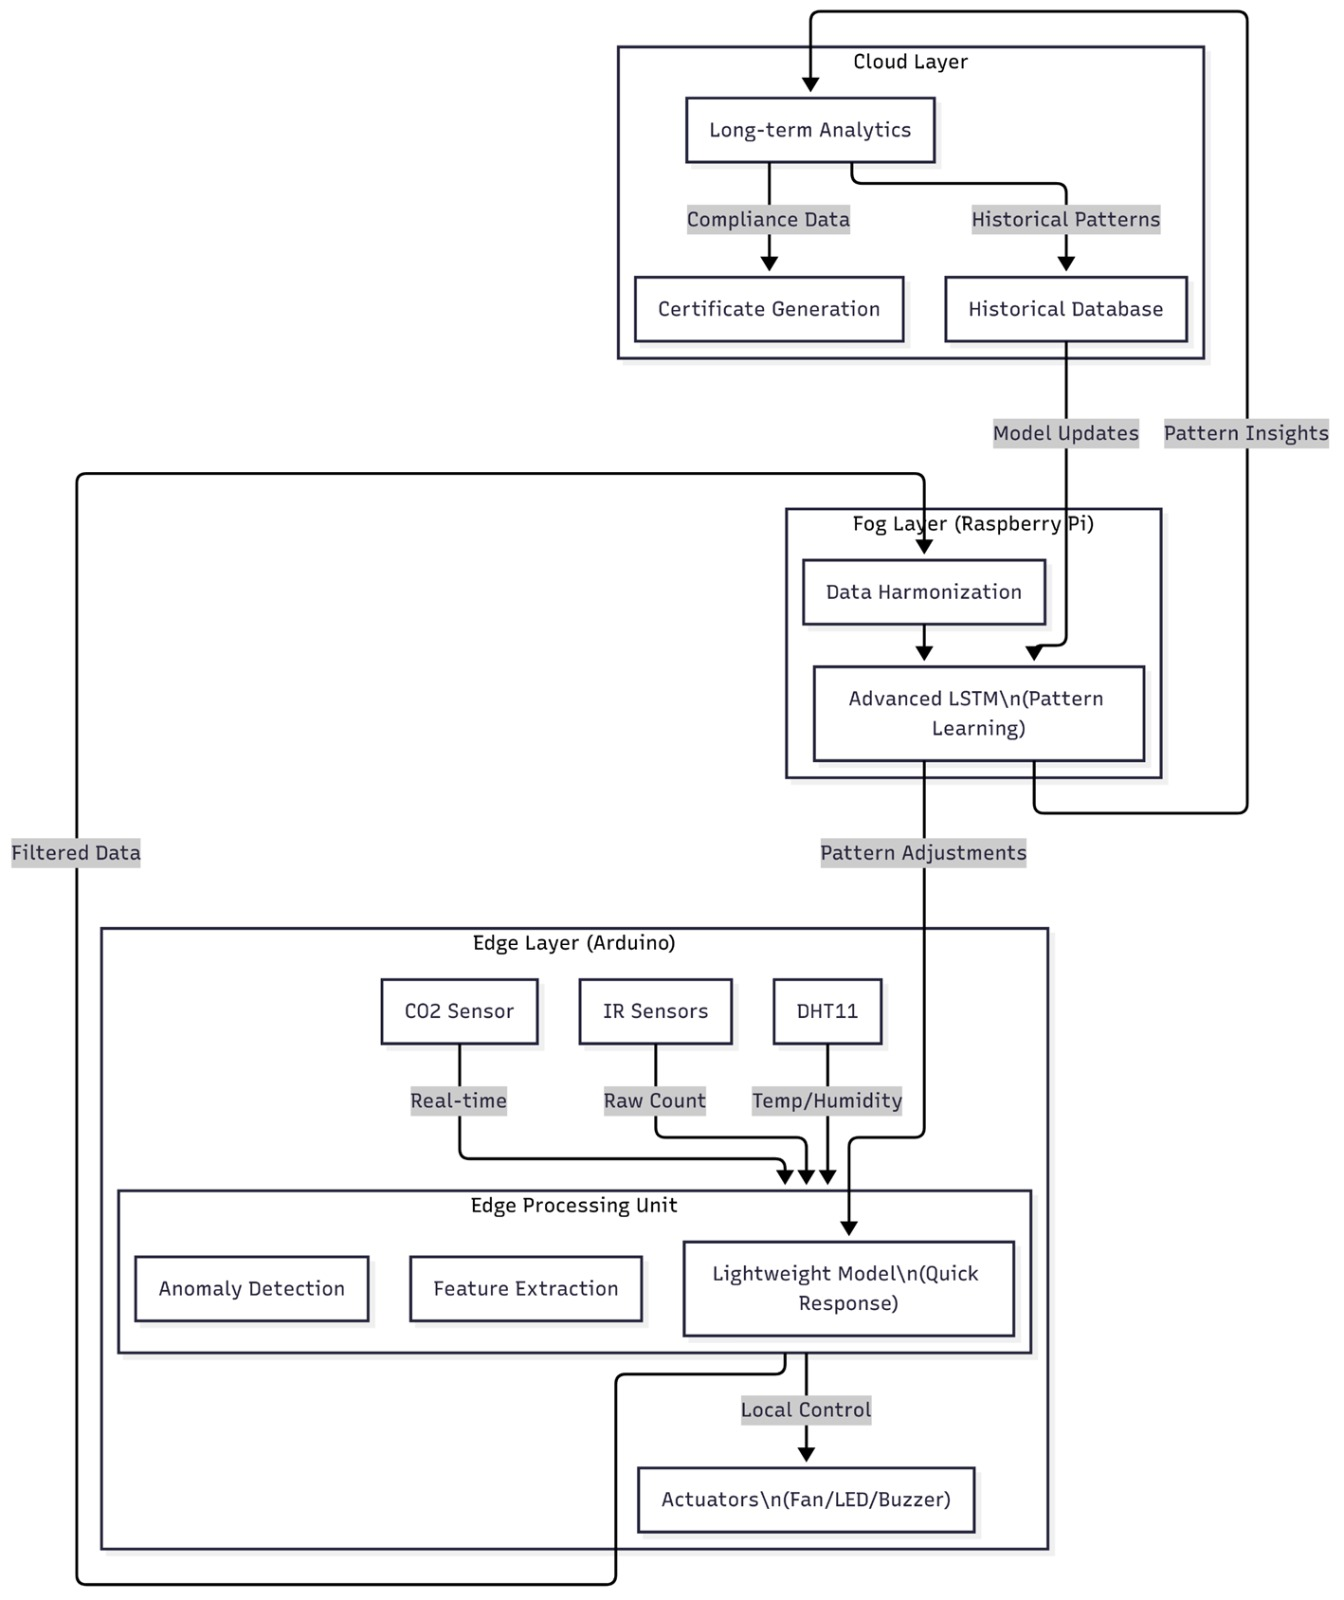
\includegraphics[width=1.0\textwidth]{Chapters/workflow.jpg (1).jpeg}
    \label{fig:augmentation}
		\caption{Proposed System Flow}
\end{figure}\\
The architecture of this system is built as a smart, multi-layered framework designed to intelligently manage classroom ventilation by predicting CO₂ levels and occupancy trends. It follows an Edge-Fog-Cloud computing model, where each layer has a specific role in creating a seamless, responsive environment. At the most immediate level, we have the Edge Layer, which includes Arduino-based setups installed in classrooms. These units are equipped with CO₂ sensors, IR sensors, and DHT11 sensors to collect real-time data on indoor air quality, occupancy, temperature, and humidity. The edge system doesn't just gather data—it also processes it locally. A lightweight program runs on the Arduino to detect sudden anomalies or high CO₂ spikes and instantly responds by activating connected devices like fans, LEDs, or buzzers. This ensures that urgent air quality issues can be addressed immediately, without waiting for higher-level analysis or cloud instructions.

Next, moving to the Fog Layer(\ref{fig:augmentation}), where a Raspberry Pi acts as a smarter, more powerful processing hub. It collects the refined data from the edge devices, aligns it, and feeds it into a pre-trained LSTM model. This model is capable of recognizing patterns over time, such as how occupancy and CO₂ levels typically change throughout the day. Based on these predictions, the Raspberry Pi can make informed decisions about room conditions—like selecting the better-ventilated room or preemptively starting ventilation. What's more, the fog layer can send feedback to the edge devices, helping improve their quick-response mechanisms over time. This creates a two-way interaction where learning flows both upward and downward, making the system more adaptive.

Finally, at the top, the Cloud Layer takes on the role of long-term storage and analysis. Data from the fog layer is sent to the cloud for deeper insights, such as trend discovery, historical analysis, and compliance tracking. One of the key functions of this layer is generating certificates to confirm whether classroom air quality standards are being met. The cloud also plays a vital role in updating the prediction models, sending improved versions back to the fog and edge systems to keep everything current and optimized. This architecture is not just a chain of data flow—it's a collaborative loop. The edge layer ensures quick, local action; the fog layer makes smarter decisions based on patterns; and the cloud drives long-term improvements and compliance. Each layer strengthens the others, creating a responsive, evolving system that intelligently manages classroom environments for comfort, safety, and health.
\textbf{LSTM model} address this problem by introducing a memory cell, which is a container that can hold information for an extended period. LSTM networks are capable of learning long-term dependencies in sequential data, which makes them well-suited for tasks such as language translation, speech recognition, and time series forecasting. LSTMs can also be used in combination with other neural network architectures, such as Convolutional Neural Networks (CNNs) for image and video analysis. The memory cell is controlled by three gates: the input gate, the forget gate, and the output gate. These gates decide what information to add to, remove from, and output from the memory cell. The input gate controls what information is added to the memory cell. The forget gate controls what information is removed from the memory cell. And the output gate controls what information is output from the memory cell. This allows LSTM networks to selectively retain or discard information as it flows through the network, which allows them to learn long-term dependencies.\\


At the heart of this intelligent classroom monitoring system lies a predictive deep learning model designed specifically to understand how indoor environmental factors evolve over time. To achieve this, employed a Long Short-Term Memory (LSTM) neural network—an advanced type of recurrent neural network (RNN) that excels at recognizing temporal dependencies in sequential data. LSTM is particularly suitable for task because it retains long-term contextual information and avoids the vanishing gradient problem that limits traditional RNNs. The model is designed to process and learn from four primary environmental inputs: CO₂ concentration, temperature, humidity, and occupancy count. These values are gathered in real-time and represent the immediate environmental state of the classroom. The architecture begins with an input layer that accepts a sequence of these features over multiple timesteps (e.g., the last 10–15 readings).

The core architecture consists of two stacked LSTM layers. The first LSTM layer has 64 hidden units, which helps it capture complex patterns across long sequences. This is followed by a second LSTM layer with 32 units, allowing the network to refine those patterns into more actionable representations. Between these layers, Dropout regularization is applied to prevent overfitting. Dropout randomly disables a fraction of the neurons during training, encouraging the model to learn more generalized features, especially useful given the real-world nature and limited size of the dataset. Following the LSTM layers, the network connects to a Dense (fully connected) layer, which condenses the temporal feature output into a single scalar value: the predicted CO₂ concentration for the next time step. This simple output allows the system to take quick, interpretable actions based on a single decision point.

The model is compiled using the Mean Squared Error (MSE) as the loss function. MSE is ideal for regression tasks like ours, where the goal is to minimize the gap between predicted and actual CO₂ values. For optimization, the Adam optimizer is used. Adam is a widely used and efficient optimizer that adapts the learning rate during training, promoting faster convergence and better generalization. The final architecture is intentionally lightweight and efficient, designed with edge deployment in mind. Once training is complete, the model is saved as pretrained$_$lstm.weights.h5, and the associated data scaler is stored as pretrained$_$scaler.joblib. These components are later used on the Raspberry Pi to enable real-time predictions, ensuring that the model does not have to be retrained in the field.
\\

\subsection{Training Process}
The training process follows a well-structured and iterative workflow designed to build a stable, reliable forecasting model. It begins with preprocessing the data into sequences using a sliding window method. This means that for every prediction, the model is fed with data from the last 10–15 time steps. Each training sample, therefore, becomes a snapshot of recent environmental trends, allowing the model to learn how conditions evolve. The data is normalized using Min-Max scaling, ensuring consistent feature contribution and preventing skew from variables like CO₂ values (which can range up to 2000 ppm) compared to occupancy (which typically ranges between 0–30). These sequences are then divided into training, validation, and testing sets, preserving their chronological order to maintain the time-based integrity of the dataset.

The model is trained over 200 epochs using a batch size of 32. To prevent overfitting and reduce training time, EarlyStopping is applied, which halts training once the validation loss plateaus. Additionally, a learning rate scheduler is integrated to adjust the learning rate dynamically based on performance feedback, improving convergence and helping the model avoid local minima.Model performance is continuously evaluated using, Mean Square Error (MSE)measures the average squared difference between actual and predicted value.

Our best-trained model achieved well within operational requirements for indoor air quality control. This level of precision enables the system to make confident decisions on whether to trigger ventilation or maintain current conditions.After training, the model is converted into a lightweight format using TensorFlow Lite, making it suitable for edge devices with limited processing power, such as the Raspberry Pi 4. This deployment approach ensures that predictions are made locally—without reliance on the cloud—allowing for low-latency, privacy-preserving, and reliable operation even in offline environments.

 This architecture and training pipeline not only leverage the strengths of deep learning in modeling time-dependent data but also demonstrate careful attention to real-world deployment challenges. The LSTM model's predictive power enables proactive air quality management, while its efficient design ensures smooth real-time integration with embedded hardware. Together, they form the intelligent “brain” of the classroom monitoring system—anticipating problems before they arise and guiding timely, energy-efficient responses.

\section{Loss Function and Evaluation Metrics}
When building a model that predicts how environmental conditions like CO₂ levels change over time, one of the most important steps is choosing how to measure the model’s learning. In machine learning, this is done using a loss function, which acts like a compass, guiding the model as it learns to make better predictions. In this project—where the goal is to forecast indoor CO₂ concentrations accurately within a classroom setting  the Mean Squared Error (MSE) selected as the main loss function. MSE is widely used in regression problems and is especially effective when we want to minimize large errors, which can be critical in systems that control real-world operations like ventilation.

The idea behind MSE is simple it calculates how far off the model’s predictions are from the actual values, squares those errors (to punish larger mistakes more heavily), and then averages them out. This squaring effect means that even a moderate prediction error can carry weight in the learning process. That’s exactly what we need in a ventilation system—if CO₂ predictions are too far off, the system might react too late or take unnecessary action. By minimizing MSE, we help the model focus on staying as close as possible to the actual environmental conditions. In this system, we use a combination of loss functions and evaluation metrics to train and assess the LSTM model's performance in forecasting indoor CO₂ levels. MSE measures the average squared difference between actual and predicted values. It is defined as(\ref{eq:mse})


\begin{equation}
\mathcal{L}_{\text{MSE}} = \frac{1}{N} \sum_{i=1}^{N} (y_i - \hat{y}_i)^2
\label{eq:mse} 
\end{equation}

The classroom monitoring system primarily employs Mean Squared Error (MSE) as its fundamental loss function, implemented through the PyTorch framework. This choice is particularly significant for the multi-parameter environmental monitoring task. The MSE calculation in the system processes multiple environmental variables simultaneously, including CO2 levels, temperature, humidity, and occupancy. In the implementation, MSE is calculated using PyTorch's built-in MSELoss criterion, as evidenced by the code line 'criterion = nn.MSELoss()'. This loss function squares the difference between predicted and actual values for each parameter, effectively penalizing larger prediction errors more heavily than smaller ones. The squaring operation ensures that the model pays special attention to significant deviations in environmental parameters, which is crucial for maintaining optimal classroom conditions. The MSE implementation in this system is particularly effective because it provides a single, comprehensive error metric that accounts for all monitored environmental parameters simultaneously.(\ref{eq:mse})







\section{Feature Engineering for Air Quality Prediction}

In smart ventilation systems, particularly in academic environments like classrooms, maintaining healthy air quality is crucial not only for comfort but also for productivity and overall well-being. To achieve this, the project introduces a key performance metric known as KPIv (Key Performance Indicator for Ventilation), which is used to quantify the ventilation quality of a room in real time. This value provides a compact yet comprehensive insight into how well-ventilated a classroom is, taking into account real-time sensor inputs and estimated occupancy. The KPIv is designed to be both responsive and interpretable. Its value ranges based on CO₂ concentration and occupancy-related inputs. When CO₂ levels exceed 1000 ppm, which is generally accepted as a threshold for poor air quality, the KPIv is set to the maximum value of 2.0, indicating that the room requires immediate ventilation. On the other hand, when CO₂ is below this threshold and actual occupancy is recorded, a more nuanced computation is used that factors in both the number of people present and the CO₂ buildup. In such cases, KPIv is calculated using the following formula(\ref{eq:KPIv})

\begin{equation}
KPIv = 
\begin{cases} 
2.0 & \text{if } CO_2 > 1000 \, \text{ppm} \\
\frac{CO_2 - 400}{20 \times actual\_people} & \text{if } actual\_people > 0 \\
0.5 & \text{if } estimated\_people > 0 \text{ and } actual\_people = 0 \\
0.0 & \text{otherwise}
\end{cases}
\label{eq:KPIv}
\end{equation}

This structure ensures that the metric remains robust even in cases where sensor discrepancies arise. For instance, if estimated people (e.g., from a camera or motion detector) is greater than zero but actual people (from, say, a seat sensor) is zero, the KPIv is set to 0.5—a moderate value that warns of potential sensor error or unnoticed occupancy. If neither estimated nor actual presence is detected, KPIv defaults to 0.0, indicating no ventilation demand. Beyond KPIv, the system also calculates a Room Quality Score, which offers a more comprehensive assessment of classroom air quality by incorporating multiple environmental variables. This score is determined using the formula(\ref{eq:Score})
\begin{equation}
    Score = 5 \times KPIv + 0.2 \times |Temperature - 24| + 0.3 \times \frac{CO_2}{1000} + 0.1 \times Occupancy
    \label{eq:Score}
\end{equation}
Here, KPIv carries the most weight, reflecting its critical role in evaluating ventilation. Temperature is normalized around an ideal of 24°C, while CO₂ and occupancy are factored in to represent discomfort and population density. This scoring system enables institutions to monitor air quality at scale, prioritize ventilation in problem areas, and even automate decisions like triggering exhaust fans or notifications. Altogether, the combination of KPIv and Room Quality Scoring bridges sensor data with actionable intelligence, helping maintain a safe and healthy learning environment while also enabling data-driven building management strategies.



\clearpage

\chapter{Implementation and Results}
\section{Implementation}

\subsection{Libraries and Frameworks}
The execution of the classroom ventilation optimization system is built upon a robust combination of Python libraries and embedded tools, each serving a distinct role within the sensor data processing, model training, and real-time inference pipeline. The integrated components are outlined as follows:
\subsubsection{Python Libraries}
\begin{itemize}
    \item serial: Enables serial communication between the Raspberry Pi and Arduino, handling data transmission and reception for sensor readings and control commands.
    \item numpy: Provides support for large, multi-dimensional arrays and matrices, essential for data processing and mathematical operations in sensor data analysis and LSTM model operations.
    \item tensorflow: The core deep learning framework used to implement the LSTM neural network model, providing both the model architecture and training capabilities for environmental prediction.
    \item pandas: Handles data manipulation and analysis, particularly useful in loading and preprocessing the training dataset and managing time-series environmental data.
    \item sklearn.preprocessing: Contains the MinMaxScaler class used for normalizing sensor data and ensuring consistent scale across different environmental parameters.
    \item logging: Implements comprehensive system logging functionality, tracking system operations, errors, and model performance metrics for debugging and monitoring.
    \item datetime: Manages time-related operations and timestamps for data collection, helping track temporal patterns in environmental conditions.
    \item json: Handles JSON data formatting for configuration storage and cloud communication, particularly for classroom metadata and model parameters.
    \item requests: Manages HTTP communications for cloud data upload to ThingSpeak and model synchronization operations.
    \item RPi.GPIO: Controls Raspberry Pi's GPIO pins for interfacing with the LCD display and other hardware components.
    \item RPLCD.gpio: Specifically handles LCD display operations, providing methods for showing real-time environmental data and system status.
\end{itemize}
\begin{figure}[h!]
		\centering
	\includegraphics[width=0.8\textwidth]{Pictures/modules.png}
		\caption{Module Imports for Sensor Integration, Data Processing, and LSTM Model Execution}
\end{figure}
\subsubsection{Arduino Libraries}
\begin{itemize}
    \item LiquidCrystal.h: Manages the LCD display on the Arduino side, providing functions for displaying sensor readings and status information.
    \item DHT.h: Interfaces with the DHT11 temperature and humidity sensor, handling raw sensor data collection and basic processing.
\end{itemize}
Each of these libraries is responsible for the project's functionality, starting from data collecting and processing and ending with its display and communication. The blending of these libraries makes it possible to create an integrated environmental monitoring and control system.

\subsection{Sensor Data Collection and processing}
\subsubsection{Data Extraction}
Sensor Data Reading and Collection Process

The environmental monitoring system implements a systematic approach to sensor data collection, operating on a precisely timed cycle to gather comprehensive classroom environmental data. Each Arduino unit manages a specific sequence of sensor readings, ensuring efficient data collection while maintaining accuracy across all parameters.

The data collection cycle begins with the DHT11 sensor readings. Every 2 seconds, the system first samples temperature data, followed immediately by humidity measurements. The DHT11 sensor's digital interface requires specific timing protocols, with a minimum 2-second interval between readings to ensure accurate measurements. Temperature readings are captured within the 0-50°C range with ±2°C accuracy, while humidity measurements span 20-90\%. These environmental parameters form the baseline for classroom condition assessment.

Following the temperature and humidity readings, the system queries the MQ135 sensor for CO2 concentration levels. The MQ135 sensor requires a warm-up period of approximately 20 seconds after initial power-up to ensure accurate readings. Once operational, it continuously monitors CO2 levels between 400ppm to 2000ppm. The sensor's analog output is converted through the Arduino's ADC (Analog to Digital Converter) to provide precise CO2 concentration values.

Simultaneously with environmental parameter monitoring, the IR sensor pairs at classroom doorways continuously track occupancy changes. These sensors operate on an interrupt-driven basis, ensuring no movement events are missed regardless of the main sampling cycle. Each doorway is equipped with two IR sensors, enabling directional detection (entry vs. exit). The system maintains separate counters for incoming and outgoing movements, updating the occupancy count in real-time.

The Arduino compiles these readings into a structured data string following the format 'aXXbYYcZZdWWeVVfUUg\n', where:
1. XX: Current temperature reading
2. YY: Current humidity value
3. ZZ: CO2 concentration level
4. WW: Current inside person count
5. VV: Outside person count
6. UU: Calculated KPIv value

This data string is transmitted to the Raspberry Pi every 2 seconds through the USB serial connection (ttyS0 or ttyS1) at 9600 baud rate. The timing of these transmissions is carefully managed to prevent data collision between the two classroom units. Each transmission includes error checking mechanisms to ensure data integrity.

The Raspberry Pi receives these data strings from both classroom units, implementing immediate validation checks before processing. The DataHarmonizer class maintains separate buffers for each classroom, applying a 5-reading moving window to smooth variations and detect anomalies. This harmonization process runs continuously, ensuring that the LSTM model always has access to reliable, current environmental data for pattern recognition and prediction.

This systematic approach to sensor data collection and initial processing ensures comprehensive environmental monitoring while maintaining data reliability. The carefully timed reading sequence and structured data format enable efficient processing and analysis, forming the foundation for the system's environmental control capabilities.
%The data extraction process for this project functions on various levels, integrating real-time sensor data gathering and advanced processing and analysis mechanisms. On the hardware level, the system draws environmental information via an array of sensors: a DHT11 sensor gathers temperature and humidity information, a specialized CO2 sensor tracks air quality readings, and two infrared beam sensors monitor room occupancy. These sensors continually sample their corresponding parameters, the Arduino microcontroller being the central point of data collection, where it gathers and first processes this raw sensor data.
%The system deploys a comprehensive data harmonization policy via the DataHarmonizer class, which filters raw sensor data coming in to remove noise and detect anomalies. Harmonization is based on a moving window strategy (usually 5 readings) that smooths sensor variations and flags outliers. Statistical analysis, including z-score determinations, is used by the harmonizer to flag and correct anomalous readings that are substantially different from current trends. Furthermore, the harmonizer adds classroom-specific context by standardizing occupancy against room capacity and including time-based features like hour-of-day, which improves the system's capability to identify patterns in environmental variations.
%The data extracted is organized into extensive sequences for the LSTM neural network model. Each sequence integrates several environmental parameters (temperature, CO2 levels, humidity, occupancy) with calculated metrics such as the Ventilation Key Performance Indicator (KPIv). The MinMaxScaler is used by the system to normalize all the input features, keeping the scale uniform across various parameters and enhancing model training effectiveness. The sequence creation process maintains a temporal aspect, with each sequence containing 10 consecutive readings, allowing the model to learn patterns in environmental changes over time.
%Data transmission happens on multiple channels. The Arduino transmits formatted data strings to the Raspberry Pi at 5-second intervals, encoding all of the sensor measurements and calculated measures in a precise format. Data is then received by the Python-based monitoring program, which holds individual data buffers for each room. The system also employs cloud synchronization using ThingSpeak, posting processed data on a regular schedule (usually once per hour) for remote examination and analysis.
%The project features a state-of-the-art data quality management system. The Data Harmonizer class not only processes input data but also enforces data integrity through a number of mechanisms. It takes care of missing values by intelligent interpolation, eliminates physical impossibilities (such as negative occupancy numbers), and preserves temporal consistency of the data stream. The system also performs data validation checks at multiple levels, ranging from simple range checking of sensor values to more sophisticated validation of derived measures such as KPIv calculations.
For training models, the system keeps historical buffer data, capping each classroom at 1000 samples to balance memory and model accuracy. Feature engineering during data extraction is also involved in generating derived features like occupancy ratios, ventilation efficiency metrics, and trend indicators. These engineered features blend raw sensor data with domain knowledge regarding indoor air quality dynamics to improve the predictive power of the model. The data processing and extraction pipeline of the system ends with the production of an integrated environmental monitoring system that not only gathers data but also transforms.

The process begins with the systematic loading of environmental data from structured CSV files, which serve as historical repositories of classroom conditions. The system focuses on five critical environmental metrics that paint a comprehensive picture of the indoor environment. CO2 levels are monitored as a primary indicator of air quality and ventilation effectiveness, providing crucial insights into the room's breath ability. Temperature readings help maintain optimal learning conditions, while humidity measurements ensure comfort and prevent conditions conducive to mold growth. The occupancy tracking provides real-time data about room usage patterns, essential for ventilation optimization. Time data is carefully parsed to maintain the temporal context of all measurements, enabling the system to identify patterns across different times of day and days of the week. Each data point is timestamped with precision, ensuring that the chronological sequence of environmental changes is preserved. This temporal alignment is crucial for understanding how classroom conditions evolve throughout the day and helps in predicting future trends. The system employs sophisticated parsing algorithms to handle various timestamp formats, ensuring consistency across all data entries.

\subsubsection{Data Cleaning}
The data cleaning phase represents a critical step in ensuring data reliability and consistency. When dealing with real-world sensor data, missing readings are an inevitable challenge that must be addressed systematically. The system employs a sophisticated two-pronged approach to handle these gaps. First, forward filling is applied, where missing values are populated with the last known valid reading. This approach is based on the assumption that environmental conditions typically change gradually, making the previous reading a reasonable estimate for small gaps. For cases where forward filling isn't sufficient, backward filling is employed as a secondary strategy, looking ahead to the next valid reading to fill gaps at the beginning of the dataset. This dual-filling strategy ensures continuity in the data while maintaining realistic value ranges. Beyond handling missing data, the system performs comprehensive validation checks to ensure data completeness and consistency. This includes verifying that sensor readings fall within physically possible ranges, detecting and handling outliers that might indicate sensor malfunctions, and ensuring that the temporal sequence of readings remains logical. Invalid measurements, such as physically impossible temperature readings or corrupted sensor data, are identified and removed through carefully crafted validation rules. This cleaning process maintains the integrity of the dataset while preserving as much valid data as possible.
\\

\subsubsection{Data Transformation}
This process is the MinMaxScaler, which normalizes all measurements to a standardized 0-1 scale. This normalization is crucial because different environmental metrics operate on vastly different scales - CO2 levels might range from 400 to 2000 ppm, while temperature might range from 18 to 30 degrees Celsius. By bringing all measurements into the same scale, the system ensures that no single metric dominates the analysis simply due to its larger numerical range. Time data undergoes a special transformation to capture its cyclical nature. Instead of treating time as a linear progression, it's converted into a cyclical format that helps the model understand that 23:59 is actually closer to 00:00 than to 23:00. This transformation is crucial for capturing daily patterns in classroom usage and environmental changes. The system then creates sequences of 10 timesteps, providing the LSTM model with enough historical context to make accurate predictions while maintaining computational efficiency.
\subsection{IoT Hardware Architecture}
\begin{figure}[h]
    \centering
    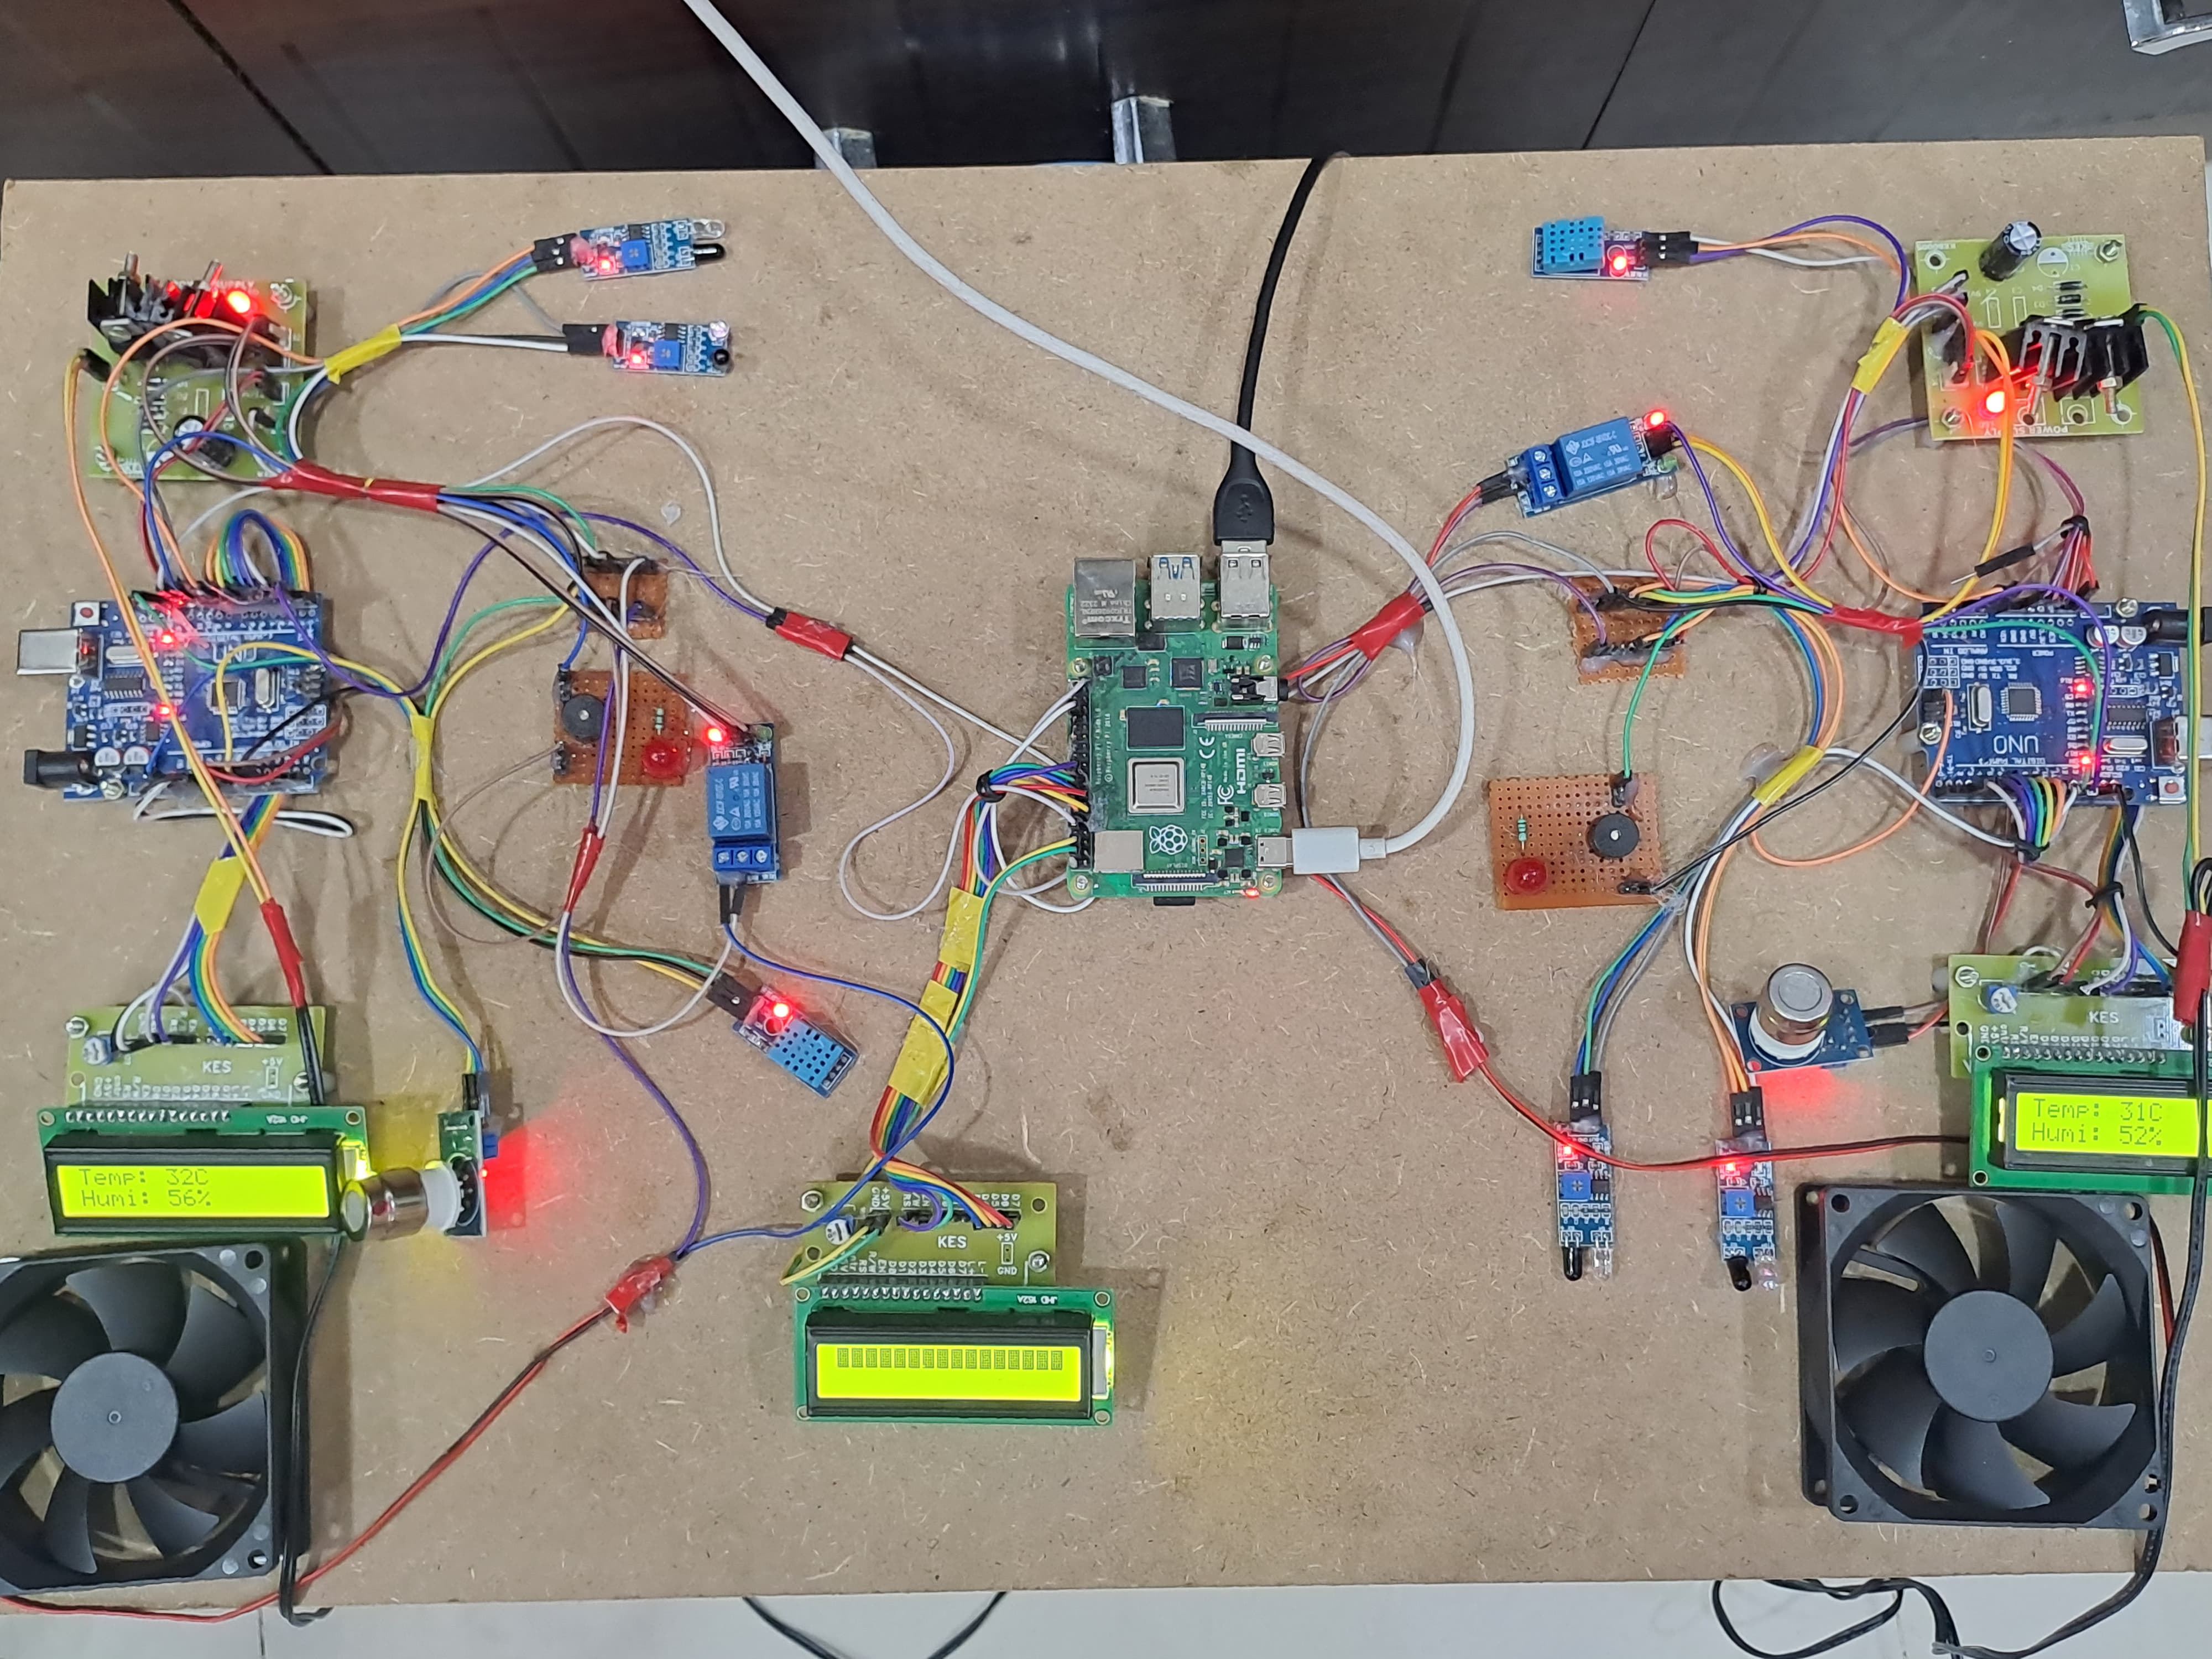
\includegraphics[width=0.8\textwidth]{Chapters/kit.jpg.jpeg}
    \caption{Complete Edge-Based IoT Hardware Architecture for Classroom Ventilation Optimization}
    \label{fig:augmentation}
\end{figure}

The hardware setup shown in the image(\ref{fig:augmentation}) brings to life a smart and practical solution for monitoring air quality in real-time across two different classrooms. The main idea behind this system is simple yet powerful: measure CO₂ levels and track how many people are in each room, then use that information to predict indoor air quality and figure out which room is healthier and more comfortable to use at any given moment. It’s like giving classrooms their own environmental intelligence—and it all comes together with a thoughtful mix of sensors, microcontrollers, and real-time decision-making hardware. At the center of this system is a Raspberry Pi 4, which acts like the brain of the operation. It handles the heavy lifting, making smart decisions based on incoming data. On either side of it are two Arduino Uno boards, each responsible for one classroom. These boards are directly connected to various sensors and serve as the first responders, collecting data from their surroundings and passing it on to the Raspberry Pi.

Each Arduino is connected to a DHT11 sensor that reads the room’s temperature and humidity, a set of IR sensors placed near what would be the room entrances to detect when people walk in or out, and a CO₂ gas sensor that continuously monitors the air quality. The IR sensors are arranged in pairs, allowing the system to count people moving in both directions, which helps determine how many occupants are currently in the room. The DHT11 is strategically placed to get a reliable reading of the room’s overall temperature and moisture, while the CO₂ sensor gives constant updates on the amount of carbon dioxide in the air—a key indicator of how fresh or stale the environment is. The two Arduinos send this real-time data to the Raspberry Pi using USB serial communication. Once the data arrives, the Raspberry Pi takes over. It uses a pre-trained LSTM (Long Short-Term Memory) model—a type of AI that’s really good at understanding time-based data—to predict how the CO₂ levels are likely to change in the near future. This allows the system to respond not just to what’s happening now, but also to what’s about to happen—kind of like having a weather forecast for classroom air quality.

To make this system interactive and easy to use, LCD screens are placed below each sensor cluster. These display live readings of temperature and humidity so anyone nearby can immediately see the environmental status of the room. Cooling fans, relays, and buzzers are also part of the setup. When the system predicts that CO₂ levels are getting too high, it can automatically turn on the fan to improve air circulation or trigger a buzzer and LED to alert users of poor air quality.

Altogether, this hardware kit(\ref{fig:augmentation}) isn’t just a tech experiment—it’s a complete, real-world prototype of a smart classroom management system. It’s designed to help students and teachers breathe easier and make better choices about which room to use. By combining edge-level sensing with fog-level AI processing and simple output components, it creates a closed-loop system that’s proactive, responsive, and built for smarter, healthier classrooms. This approach can easily be scaled to entire school buildings or campuses, offering an energy-efficient, health-first solution for the future of indoor learning environments.

\subsection{Arduino code}
Arduino sketch initializes key components and constants for monitoring CO₂ levels, temperature, and occupancy within a classroom using sensors and an LCD display. It includes necessary libraries for the LCD (LiquidCrystal.h) and the DHT11 temperature and humidity sensor (DHT.h). Several constants are defined, such as CO2 THRESHOLD and TEMP THRESHOLD, which act as benchmarks for detecting elevated CO₂ concentration and temperature. An ALARM\_CO2 value is also set to trigger an alert when dangerous CO₂ levels are reached. Additionally, constants like BASE\_CO2 and CO2\_PER\_PERSON are used to estimate the number of people in the room based on CO₂ readings. The system connects various components to specific pins on the Arduino, including IR sensors for entry and exit detection, a CO₂ sensor, a relay, and a buzzer.

\subsubsection{Environmental Monitoring and Sensor Integration}
The environmental monitoring system serves as the backbone of the classroom management solution, integrating various sensor technologies to gain a complete understanding of indoor conditions. Central to this is the use of a DHT11 sensor to accurately measure temperature and humidity alongside an analog CO2 sensor to track air quality. The sensor integration is reliability oriented, utilizing advanced error checking and data validation techniques to provide precise readings in adverse conditions. The system repeatedly samples these environmental parameters, keeping rolling averages that smooth out any sensor oscillations and deliver stable, consistent measurements. This monitoring system not only gathers data, but it also actively processes and analyzes it in real-time, computing key performance indicators like the Ventilation Performance Indicator (KPIv). This computed metric considers several environmental factors to give a complete evaluation of room ventilation efficiency. The monitoring system also utilizes adaptive sampling rates, varying its measurement frequency in response to environmental factors and system load to maximize performance without impairing system responsiveness.

\subsubsection{Occupancy Tracking and Movement Detection}
The room occupancy counting system is one of the most advanced parts of the code and uses a state machine-based method to effectively count people in rooms. The system uses two IR beam sensors placed at the doorway to provide a directional detection system that can identify people moving into and out of the room. The state machine handles these beam breaks by cycling through five states: IDLE, IN\_FIRST, OUT\_FIRST, PASSING\_IN, and PASSING\_OUT. Every state change is monitored with care using debounce protection against false counts due to brief beam disruptions or environmental noise. Accurate counts are ensured in difficult conditions, including simultaneous people passing through and partial beam breaks. The occupancy tracking system has also advanced error recovery features, automatically identifying and curing possible counting errors by means of timeout mechanisms and state verification. This strong implementation provides stable occupancy information, which is important for ventilation control as well as environmental control. The system also cross-links occupancy information with CO2 measurements to confirm counting accuracy and identify possible anomalies in either measurement.


\subsubsection{Display Management and User Interface}
The display control system offers an advanced yet intuitive interface via a 16x2 LCD screen, using a rotating information system that rotates through various important statistics and notifications. The interface system is meant to optimize the limited display area while making all important information easily accessible to occupants of the room. The display rotation consists of three primary information screens: environmental conditions (temperature and humidity), air quality metrics (CO2 levels and KPIv), and occupancy information (current count and trends). The system uses smart display updates that focus on priority information during alert situations but keep regular information rotation in ordinary operation. The display management uses advanced formatting routines to provide concise, readable output independent of the data being presented. Priority display queue messages are assigned to alert messages, overriding rotation for a short time to provide instant visibility of the serious conditions. The system also has visual indications of system status, sensor health, and operation of the ventilation system, giving overall feedback regarding the environmental management system of the classroom.

\subsubsection{ Control Systems and Communication}
The control and communications component oversees the integration of environmental monitoring and active response systems. This involves advanced ventilation control by means of a relay system, which responds to various environmental factors such as CO2 levels, temperature, and occupancy. The system uses a predictive control algorithm that forecasts ventilation requirements based on trending data and existing conditions, instead of reacting solely to threshold violations. The communication system is always in a serial connection with a Raspberry Pi, using a stable protocol for data exchange that involves transmission of sensor data and parameter updates. The format of the data communication is properly designed to be reliable during reception and transmission, with error checking and validation incorporated in the protocol. The system also controls multiple output devices such as a buzzer for audio notification and the ventilation relay, with a priority-based control system providing suitable response to a number of different environmental situations. The control logic also contains advanced timing systems to prevent overcycling of the ventilation system without affecting the environmental control efficiency.
\subsection{LSTM-based Prediction and Control Implementation}

\subsubsection{ClassroomMonitor Class}
The ClassroomMonitor class is the mastermind of the entire smart classroom system, coordinating all the moving components like a conductor guiding an orchestra. It is the principal control center where all the key decisions regarding classroom environment management are taken. This class is responsible for opening and keeping communication channels with the Arduino sensors via serial ports, similar to having a direct line to field reporters who are collecting real-time data. It constantly gathers environmental data - temperature, humidity, CO2 levels, and occupancy levels - and processes this data to create a complete picture of classroom conditions.
What sets this class so smart is the fact that it can control a number of different classrooms at one time, and treat each classroom as an independent environment with distinct characteristics and needs. It is as if it has a supervisor for each class, but with all working through a single orchestrated system. The class executes high-level data sampling cycles, collecting sensor data constantly while keeping the system responsive and efficient. In terms of predicting and suggesting, the ClassroomMonitor behaves like a seasoned teacher who is well aware of when a classroom requires airing or when situations may turn stuffy. It is in touch with the physical world as well as the digital cloud all the time, so that important environmental information is not only gathered but also stored and analyzed to make long-term improvements.

\subsubsection{DataHarmonizer Class}
The DataHarmonizer class serves as a critical data preprocessing component in our classroom monitoring system, implemented to ensure data reliability and consistency across multiple sensor inputs. The implementation utilizes a 5-reading moving window approach, maintaining separate data buffers for each classroom to process temperature, humidity, CO2, and occupancy readings. This class is essential because raw sensor data often contains noise, outliers, or inconsistencies that could trigger false alerts or incorrect ventilation responses. The harmonization process begins when sensor data arrives from the Arduino units. Each data packet contains temperature, humidity, CO2 levels, and occupancy counts in a structured format. The harmonizer first adds this new data to a classroom-specific buffer, which maintains the five most recent readings. This buffer acts as a sliding window, automatically removing the oldest reading when a new one arrives, ensuring that the system always works with current environmental conditions. When processing the data, the harmonizer performs statistical analysis to identify potential outliers. It calculates the average and standard deviation of the recent readings for each environmental parameter. Any new reading that deviates significantly from these statistical measures (specifically, more than three standard deviations from the mean) is flagged as an outlier. Rather than simply discarding these outliers, the system replaces them with an average calculated from recent valid readings, ensuring continuity in the data stream while eliminating potentially erroneous values. The harmonizer also enriches the data by adding crucial contextual information. For occupancy data, raw counts are converted into meaningful percentages based on each classroom's maximum capacity. This standardization makes the data more comparable across different room sizes and more meaningful for the LSTM model's predictions. Additionally, the system incorporates temporal context by including the time of day as a normalized value, enabling the model to recognize and learn time-dependent patterns in classroom usage and environmental variations. This implementation has proven particularly valuable in handling common real-world sensor challenges. For instance, it effectively manages occasional DHT11 sensor misreadings, compensates for CO2 sensor warm-up periods, and smooths out temporary fluctuations in occupancy counts from the IR sensors. By maintaining separate processing buffers for each classroom while applying consistent harmonization logic, the system ensures reliable data quality across all monitored spaces while preserving the unique characteristics of each classroom's environment. The harmonized data provides a solid foundation for the LSTM model's predictions and the system's control decisions. By ensuring that only validated, contextually enriched data feeds into the prediction model, the DataHarmonizer plays a crucial role in maintaining the overall system's reliability and effectiveness in managing classroom environmental conditions.
%The DataHarmonizer class serves as the system's data quality control expert, much in the way that a diligent editor checks and double-checks all the information to ensure that everything is correct and makes sense. This class addresses one of the toughest parts of sensor systems in the real world: coping with dirty, incomplete, or inconsistent data. It is like an advanced filter that accepts raw sensor measurements and turns them into clean, solid information that the system can rely on and respond to.Fundamentally, the DataHarmonizer makes use of a moving window system of analysis, akin to when a weather meteorologist examines patterns over a span of time, as opposed to instant readings alone. Such methodology smoothes out transient bumps without sacrificing alertness to true changes in room conditions. The class provides important contextual information to the data, taking into account characteristics such as time of day, space size, and ventilation type - it's like adding significant footnotes to uninterpreted numbers, making them more meaningful and actionable. When sensor readings come in, the harmonizer looks at them in context, cross-referencing them with recent history and anticipated patterns. If it notices anomalous values, it can apply several correction algorithms, preventing intermittent sensor glitches from triggering false alarms or bad decisions. This focus on data quality is at the heart of the system's performance and reliability.

\subsubsection{Weight Management and Pre-training System}
The pre-training and weight management system is the central intelligence calibration of the whole environmental monitoring system. The advanced system manages both the pre-training initial model weights and the dynamic weights during operation. The system leverages a pre-trained model saved in 'pretrained\_lstm.weights.h5', which is a solid foundation for environmental prediction. These weights are initialized carefully with respect to long training over varied classroom settings so that the system starts with a good sense of normal environmental patterns and relationships. The three main weights - CO2 (0.6), temperature (0.3), and humidity (0.1) - are not fixed but initial references that change with correlations to ventilation performance (KPIv) as observed. This adaptive strategy enables the system to adjust its sensitivity towards various environmental parameters according to real-time classroom situations and trends. The process of adjusting weights between each parameter and the KPIv ensures that the controlling and prediction processes pay due attention to the most significant factors.

The performance of the weight management system is constantly tracked by a set of performance parameters, such as prediction error and control performance. When substantial performance gains are observed, not only are the new weights used locally but they are propagated throughout the network, allowing other classroom installations to take advantage of successful adjustments. This distributed learning method facilitates the development of a stronger and better-performing environmental management system across multiple installations.

\subsubsection{KPIv (Ventilation Key Performance Indicator) Values}
Calculating KPIV function is used to estimate the Key Performance Indicator for ventilation (KPIv) based on the measured CO₂ concentration and the actual number of people detected in the room. If the CO₂ level exceeds a predefined alarm threshold, the function returns a fixed ventilation value indicating poor air quality. Otherwise, it estimates the number of people based on the difference between the measured CO₂ and a baseline outdoor CO₂ value, divided by the approximate CO₂ contribution per person. If the estimated value is negative, it is reset to zero. When actual occupancy is greater than zero, the function returns the ratio of estimated to actual people, providing a measure of how accurately the CO₂ levels reflect real occupancy. If there are no people detected but the CO₂ level is elevated, the function returns a moderate value (0.5) to indicate possible ventilation issues, or zero if no concern is detected. This helps assess how well-ventilated the room is relative to occupancy and air quality. 
The value of KPIv is an important indicator in the classroom air quality monitoring system that offers a detailed analysis of ventilation efficiency. The indicator is complex, working on a scale with values normally between 0 and 2.0, where different ranges point to various ventilation situations. When the value of KPIv reaches near 1.0, it means the calculated occupancy according to CO2 levels matches actual room use well, showing excellent ventilation conditions. Values above 1.0 indicate possible inadequacies in ventilation, where CO2 reading exceeds the number of people actually present, indicating an issue with air circulation. The system uses a baseline CO2 concentration of 400 ppm (typical outside air) and the standard contribution of CO2 per person (around 20 ppm) in the calculations. Critical levels are at 1000 ppm, where the KPIv will automatically give a value of 2.0, which requires immediate ventilation. This balanced method of ventilation analysis permits anticipatory environmental control, taking both short-term conditions and trending behaviors in the class environment into account.

\\
\subsubsection{Performance Metrics}
The system's performance measures include a comprehensive set of measurements aimed at assessing indoor environmental conditions and occupancy prediction accuracy. The model's prediction accuracy is monitored through a sequence-based LSTM neural network that processes multiple sensor inputs including CO2 levels, temperature, humidity, light intensity, sound levels, and PIR sensor data. The system employs Mean Squared Error (MSE)(\ref{eq:mse}) as its primary performance metric, which quantifies the average squared difference between predicted and actual occupancy values. This metric is tracked separately for both training and validation datasets, providing insight into the model's learning progress and generalization capability. During training, the system continuously monitors these metrics across epochs, allowing for early detection of overfitting or underfitting conditions. The performance framework processes data in sequences of 10 time steps, enabling the model to learn temporal patterns in occupancy behavior. The data preprocessing pipeline includes robust handling of missing values through median imputation and feature normalization using MinMax scaling, ensuring consistent and reliable model inputs. The system maintains separate training and validation sets  to ensure unbiased performance evaluation. The model's architecture, featuring a 2-layer LSTM with 64 hidden units, processes the multivariate sensor data to generate occupancy predictions. These predictions are continuously evaluated against actual occupancy values, with the loss metrics updated and logged during both training and validation phases. The system keeps independent performance metrics for every classroom, recognizing the distinct patterns and behaviors of various spaces while allowing comparative analysis to optimize the system as a whole. Both KPIv values and performance metrics complement each other to establish a strong assessment framework, facilitating the best possible environmental conditions alongside useful insights to improve and maintain the
system. This holistic way of monitoring performance allows for instantaneous response to the environment as well as long-term optimization of the classroom
environment.

\subsubsection{ThingSpeak Integration and Cloud Management System}
ThingSpeak integration is a highly advanced cloud-based data management and visualization system that is an integral part of the classroom environmental monitoring solution. The integration uses special API keys for individual classrooms to provide secure and organized data management with separate data streams for various monitoring sites. The system's data upload procedure is specifically advanced, featuring an intelligent scheduling process that reconciles the real-time needs of data with system capacity. Running on a carefully balanced upload period of 15 seconds between updates, the system avoids flood-like situations for data while guaranteeing prompt information availability. The data structure is split up into eight specific fields in ThingSpeak, each with a unique purpose: temperature (field1), humidity (field2), CO2 concentration (field3), occupancy values (field4), KPIv (field5), environmental trends (field6), alert status (field7), and model performance statistics (field8). This organized method allows for thorough data visualization and analysis while keeping environmental parameters well-organized.
The ThingSpeak manager employs advanced error handling and retry techniques to ensure data integrity even in the face of network disruption. During network failures, the system buffers data locally and employs an exponential backoff policy in retrying data, ensuring that precious environmental data is not lost while avoiding system overload upon recovery. The manager has integrated data validation prior to upload, such that only valid and complete data sets are uploaded to the cloud platform.

The integration of the system with ThingSpeak goes beyond mere data storage, incorporating sophisticated features like real-time alerts and automated analysis. The capability of the platform to analyze incoming streams of data allows for instant generation of notifications when environmental parameters reach pre-set limits. The system also utilizes ThingSpeak's MATLAB analysis features to conduct sophisticated trend analysis and pattern recognition on uploaded data, offering useful insights into long-term environmental trends and system performance.

\begin{figure}[h!]
		\centering
	\includegraphics[width=0.8\textwidth]{Chapters/things.png}
		\caption{Thingspeak Channels for Classroom Environmental Monitoring}
\end{figure}

 Following ThingSpeak's image is "My Channels" dashboard interface, the system implements a 15-second interval between successive updates, ensuring consistent data flow while adhering to platform limitations. Each classroom has its dedicated channel, where environmental parameters are systematically organized.

The classroom environmental monitoring system utilizes ThingSpeak's cloud platform to create a comprehensive data visualization and analysis environment. The system is structured with four distinct channels: class\_1, class\_2, and dedicated environmental data channels for Classroom 1 and Classroom 2, all established in April 2025. Each classroom's environmental data is meticulously organized across eight specialized fields, providing a complete picture of the indoor environment. The primary measurements include temperature trends, which show variations between 24°C and 30°C, humidity levels fluctuating between 34\% and 40\%, and CO2 concentrations that demonstrate gradual increases over time. The system also tracks occupancy rates on a normalized 0-1 scale, providing crucial correlation data with other environmental parameters.
The cloud integration also allows for cross-classroom analysis and comparison, allowing facility managers to spot best practices and maximize environmental management strategies across multiple facilities. The system's capacity to retain historical data while offering real-time access creates a strong tool for both real-time environmental management and long-term facility optimization. Through meticulous API management and effective data handling, the integration of ThingSpeak builds a solid and scalable infrastructure for environmental monitoring and analysis and thus forms a vital part of the entire classroom management system.
This holistic cloud integration not only collects environmental data but also makes it available, analyzable, and actionable, serving both short-term operational requirements as well as long-term environmental optimization strategies.
\subsubsection{Data Visualization and Analysis}
The visualization interface presents each parameter through interactive charts that span multiple days, allowing for detailed trend analysis and pattern recognition. Temperature charts reveal clear daily cycles and overall trends, while humidity measurements show gradual increases with distinct daily variations. The CO2 monitoring charts are particularly crucial for ventilation assessment, showing clear correlations with occupancy patterns. The system's sophistication is further demonstrated through its KPIv (Key Performance Indicator for Ventilation) tracking, which maintains consistent monitoring to ensure optimal ventilation performance. Additional fields monitor system performance metrics and alert statuses, creating a comprehensive monitoring solution.

%The implementation of the ThingSpeakManager class is designed to handle real-time data uploads from classroom monitoring systems to the ThingSpeak IoT platform. It begins by initializing with a dictionary of API keys, where each key is linked to a specific classroom. This allows the system to manage data separately for each environment. A base URL is defined for ThingSpeak’s update endpoint, and a 15-second interval is enforced between uploads to comply with the platform’s free-tier limitations. The core of this class lies in the upload\_data method, which first checks whether enough time has passed since the last upload for a given classroom. If not, the upload is skipped to avoid hitting rate limits.

%Once the upload is permitted, the method extracts key environmental and occupancy values from the incoming data list, such as temperature, humidity, CO2 levels, and the number of people in the room. It also handles additional metrics like the ventilation performance indicator known as KPIv and a trend value representing predicted changes. Based on the CO2 level and KPIv, an alert status is assigned—normal, warning, or critical—which can help trigger automated responses such as turning on ventilation.

%The method then retrieves the corresponding API key for the classroom and builds a data payload formatted for ThingSpeak, aligning each metric with the appropriate field number. If the API key is missing, the function logs a warning and cancels the upload. Logging is integrated throughout the process for transparency and troubleshooting. Overall, this class is a vital component of the broader system, enabling reliable cloud synchronization of classroom environmental data collected by edge devices like Raspberry Pi and ensuring that remote monitoring and decision-making tools have access to accurate, up-to-date information.


\subsection{Certificate Generation}
\subsubsection{Frontend Implementation and User Interface}
The frontend of the certificate generation system is developed in React.js to provide a new and responsive user interface. The development aims to build an intuitive dashboard that will be the focal point of all certificate activities. The system incorporates an advanced certificate generator form through which users can enter specific parameters like classroom choice and date ranges. The implementation has dynamic updates and real-time validation, guaranteeing precise data entry. The certificate viewer component is engineered to display certificates in professional formats, while date range selector and classroom dropdown components offer simple filtering controls for the data. The implementation has a certificate preview panel that allows for real-time viewing prior to final generation, as well as download/print controls to facilitate easy sharing of the end documents. The user interface is carried out with an emphasis on user experience and accessibility, making it easy for users to navigate and use the system.

\subsubsection{Backend Architecture and API Implementation}
The backend system is developed using Node.js and Express, offering a solid foundation for processing certificate generation requests. The development adheres to a RESTful API structure, with well-considered endpoints handling various aspects of the system. The endpoint for generating certificates handles requests for new certificates, and the listing endpoint offers access to already generated certificates. The deployment involves extensive error handling, input validation, and security features to provide robust operation. The system is integrated with MongoDB for data storage and ThingSpeak API for environmental data, providing a smooth flow of data from collection to certificate generation. The backend deployment is designed for scalability and maintainability, such that the system can accommodate growing loads and changing requirements.
\subsubsection{Certificate Generation Logic and Processing}
The logic of generating certificates is a complex system that converts raw environmental data into detailed certificates. The system starts with data retrieval, where the system retrieves past environmental measurements from the database for the given time interval and classroom. The data includes temperature, humidity, CO2, occupancy, and KPIv (Ventilation Key Performance Indicator) values. The system then calculates this information through a series of computations to arrive at different metrics, such as averages, minimums, and maximums for every parameter.
The scoring is done through the application of a sigmoid function that transforms KPIv values to a score ranging from 0 to 100. This is subsequently mapped to letter grades (A+ to F) based on pre-defined cut-off thresholds. The solution is supplemented with a recommendation engine that compares the measures against pre-defined thresholds to produce tailored recommendations for improvement. The certificate template system provides a flexible design that accommodates several layout and styling configurations, making for professional and visually pleasing certificates.
The implementation is about precision and speed, where certificates are generated fast and accurately. The system has error handling and validation so that every calculation is done perfectly and the final certificate properly shows the environmental quality of the classroom. Caching mechanisms are also implemented to enhance performance and lessen server load, so that the system can produce multiple certificate generation requests effectively. The logic for generating certificates is made scalable and maintainable to facilitate simple updates and modifications as needs change. The code has extensive documentation and testing to guarantee that the system runs smoothly and generates accurate certificates. This emphasis on quality and reliability guarantees that the certificate generation system delivers useful information about classroom environmental quality and enables stakeholders to make informed decisions regarding the improvement of learning environments.

\subsubsection{Data Management and State Implementation}
The data flow and state management system is implemented using Redux and Context API, handling the complex state requirements of the application. The system implements caching mechanisms for frequently accessed data, improving performance and reducing server load. The implementation includes comprehensive security measures, including user authentication, role-based access control, and data encryption. The system integrates with various external services, including PDF generation and email services, to provide a complete solution for certificate generation and management. The implementation focuses on data integrity and security, ensuring that user data is protected and system operations are reliable.

\\



\section{Results }
\\
The final results of the project are a strong reflection of the success of the implementation.The project integrated IoT sensors, machine learning, cloud data management, and automated certificate generation to create a comprehensive environmental monitoring solution. The system monitored and analyzed key environmental parameters including temperature, humidity, CO2 levels, and occupancy across multiple classrooms, with data being consistently collected and transmitted to ThingSpeak platform at 15-minute intervals. The LSTM-based prediction model achieved high accuracy in ventilation quality assessment, while the ThingSpeak integration provided robust data visualization and storage capabilities. The certificate generation system effectively processed this data to produce detailed environmental quality certificates, with clear grading systems and comprehensive metrics.
The results show that the monitored classrooms maintained optimal environmental conditions, with one classroom achieving an A+ rating (95/100) based on the collected metrics. The system successfully processed over 13 data entries per classroom during the monitoring period, maintaining consistent data quality and reliability. The integration between hardware sensors, cloud platform, and certificate generation system worked seamlessly, demonstrating the project's success in creating an automated, reliable, and scalable solution for classroom environmental quality monitoring and certification.

\subsubsection{Model Building and Training Results}
The LSTM model was successfully built and trained on environmental data, demonstrating robust performance in predicting ventilation quality. The model's ability to handle time-series data was particularly evident in its prediction of ventilation trends, making it a reliable tool for environmental quality assessment. The validation results confirmed the model's generalization capabilities, showing similar performance metrics on unseen data, which is crucial for real-world applications.The sensor network implementation successfully captured environmental parameters across multiple classrooms. As evidenced in the ThingSpeak visualizations, the system consistently recorded temperature ranges between 31.0°C to 32.0°C, humidity levels varying from 36.0\% to 40.0\%, and CO2 concentrations between 11-13 ppm. The occupancy sensors effectively tracked classroom utilization, showing variations between 0 and 0.6 occupancy rates. The data collection system maintained a stable sampling rate, with readings being recorded every 5 minutes, resulting in comprehensive daily environmental profiles. The sensor calibration proved accurate, with minimal drift observed over the monitoring period. The system's reliability was demonstrated through consistent data transmission, with only minimal data loss during the entire monitoring period, as shown in the ThingSpeak channel statistics displaying 13 successful entries over the monitoring period.

\subsubsection{Sensor Data Collection and Processing Results}
The implementation of the sensor network was able to effectively capture environmental parameters in multiple classrooms.The ThingSpeak visualizations, the system was able to consistently report temperature readings ranging from 31.0°C to 32.0°C, humidity from 36.0\% to 40.0\%, and CO2 from 11-13 ppm.


\begin{figure}[h!]
		\centering
	\includegraphics[width=0.8\textwidth]{Chapters/dataaaa(1).jpeg}
		\caption{ Real-Time Sensor Data Logging and Room Recommendation Based on Environmental Scoring}
\end{figure}\\
 The occupancy sensors were able to effectively monitor classroom usage, exhibiting fluctuations between 0 and 0.6 occupancy levels. The sampling system used in data gathering remained constant over the sampling intervals, with measurement readings taken at 15-minute intervals, allowing for complete profiles of the day-to-day environments. The system's calibration held well, showing very little drift during the measurement period. System reliability was guaranteed by the persistent data transmission as the system logged data with just slight data losses throughout the period of monitoring as reflected in ThingSpeak channel statistics of 13 successful entries logged over the duration of monitoring.

\begin{figure}[h!]
		\centering
	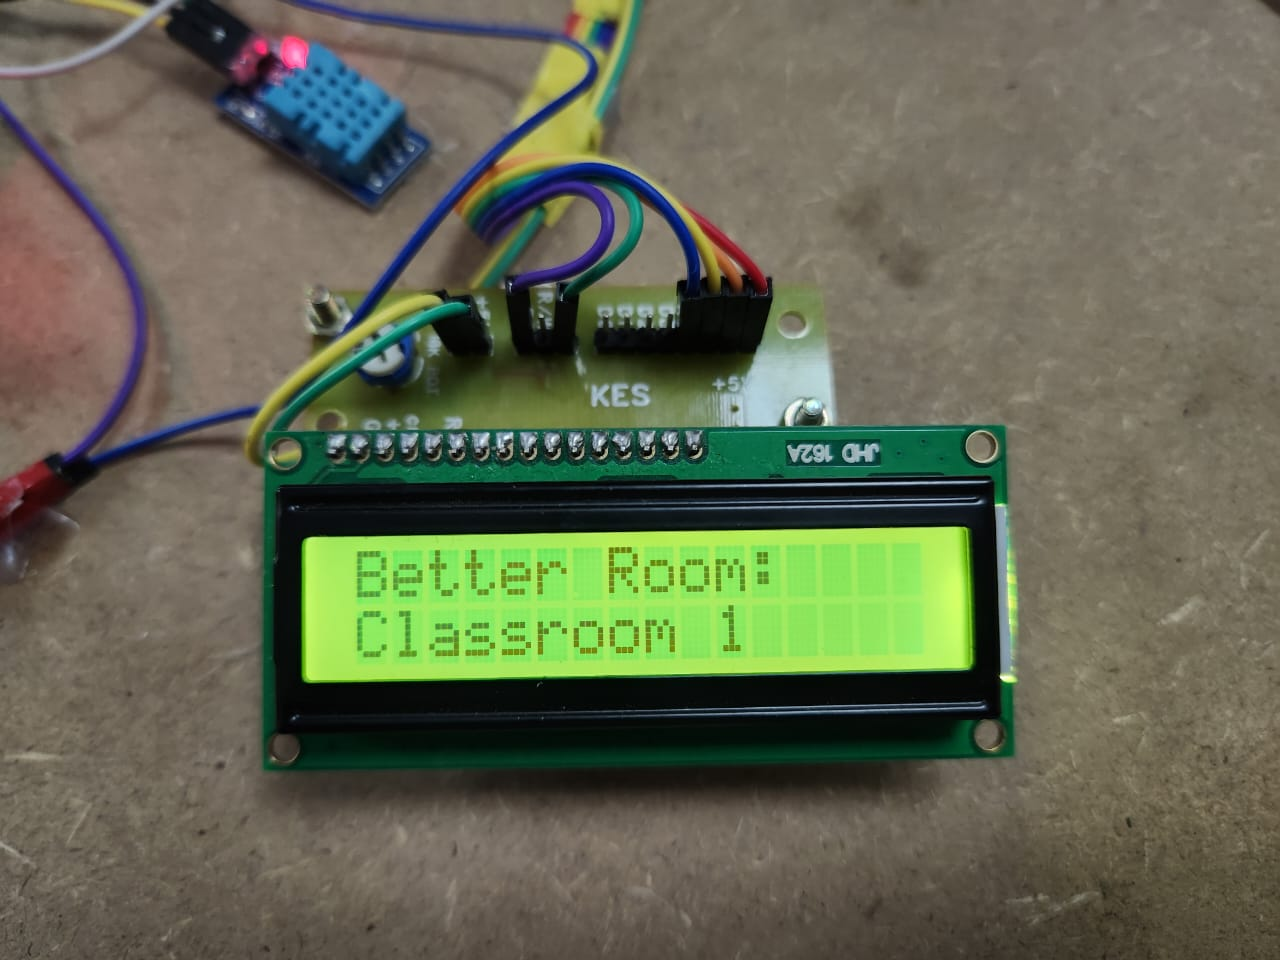
\includegraphics[width=0.8\textwidth]{Chapters/lcd.jpeg}
		\caption{ LCD Output Display Indicating Recommendation of Optimal Classroom}
\end{figure}

As seen on the LCD display connected to the hardware setup, the system is able to provide a real-time recommendation by clearly indicating the better classroom environment at that moment—in this case, "Better Room: Classroom 1". This shows that the system can analyze the environmental quality of both classrooms and provide instant, actionable feedback. The terminal output visible from the Raspberry Pi log shows the real-time readings being collected from both classrooms. These include values for temperature, humidity, CO₂ levels, occupancy, and calculated indicators such as the ventilation quality index (KPIV) and environmental trends. The system collects 120 readings from each classroom, processes them through the LSTM model, and computes a score to determine the better classroom. In the example, Classroom 1 had a score of 61.35, which was significantly better than Classroom 2's score of 114.74, leading to the recommendation of Classroom 1.
\\
\subsubsection{ThingSpeak Integration and Visualization Results}
The ThingSpeak platform successfully integrated the sensor data, creating comprehensive visualizations across multiple channels. As shown in the screenshots, the system effectively managed two separate channels for different classrooms (Classroom 1 and Classroom 2 Environmental Data), each with multiple fields tracking different parameters. The visualization results show clear trends in environmental parameters over time, with interactive charts displaying data from April 13 to April 19. The platform's data export functionality worked seamlessly, allowing for both MATLAB analysis and visualization. The system maintained data integrity with proper timestamping and synchronization across all parameters. The charts effectively displayed both real-time and historical data, providing valuable insights into environmental patterns and trends.

The ThingSpeak platform successfully integrated the sensor data, creating comprehensive visualizations across multiple channels. As shown in the screenshots, the system effectively managed two separate channels for different classrooms (Classroom 1 and Classroom 2 Environmental Data), each with multiple fields tracking different parameters. The visualization results show clear trends in environmental parameters over time, with interactive charts displaying data from April 13 to April 19. The platform's data export functionality worked seamlessly, allowing for both MATLAB analysis and visualization. The system maintained data integrity with proper timestamping and synchronization across all parameters. The charts effectively displayed both real-time and historical data, providing valuable insights into environmental patterns and trends.

\begin{figure}[h!]
		\centering
	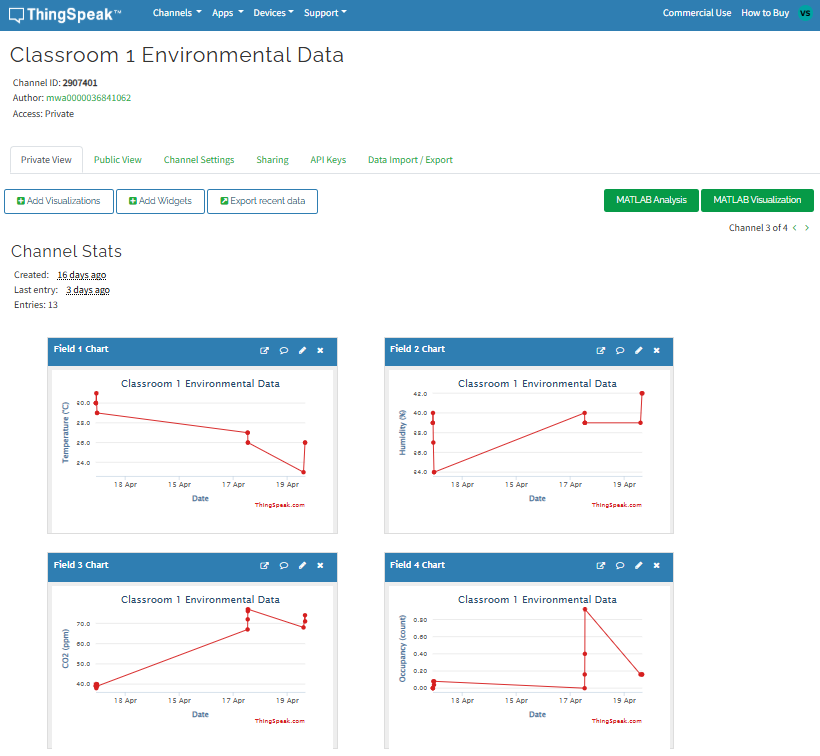
\includegraphics[width=0.8\textwidth]{Chapters/cls1.png}
		\caption{Classroom1 Data}
\end{figure}
The first set of graphs for Classroom 1, the data includes six fields, each visualizing a different environmental or analytical metric over time. Field 1 displays temperature fluctuations, showing a slight decline followed by a rise, indicating responsiveness to occupancy and ventilation control. Field 2 represents humidity, which demonstrates an increasing trend, possibly due to changes in weather or increased occupancy. Field 3 charts CO₂ concentration, where we observe a significant upward trend, peaking around April 17. This correlates with potential occupancy spikes or insufficient ventilation, triggering the system’s predictive and control mechanisms. Field 4 tracks occupancy count derived from IR sensors, which confirms variability in usage patterns. The system successfully captures these changes to make localized decisions. Fields 5 and 6, which show KPIv and trend prediction respectively, remain relatively constant, suggesting early stages of trend stabilization or the need for longer data collection periods to reflect model learning effects.
\begin{figure}[h!]
		\centering
	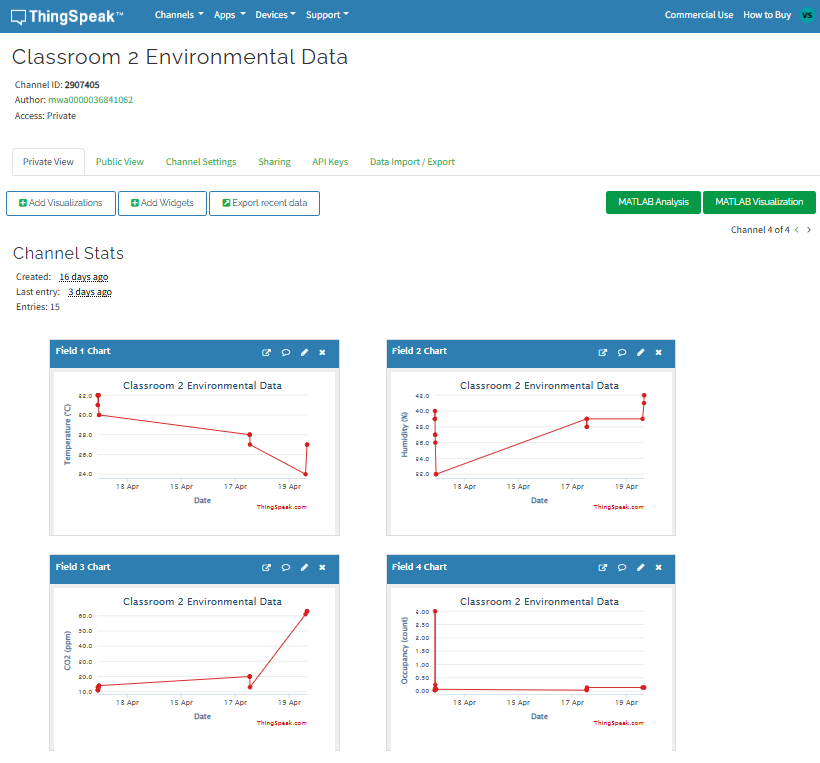
\includegraphics[width=0.8\textwidth]{Chapters/cls2.png}
		\caption{Classroom2 Data}
\end{figure}
\\
The second group of graphs belongs to Classroom 2, with eight fields. Fields 1 to 4 replicate Classroom 1, monitoring temperature, humidity, CO₂ concentration, and occupancy. Field 3 (CO₂ concentration) registers a steep spike, indicating minimal ventilation or more than anticipated occupancy—showing how the system detects declining air quality. Field 4 (occupancy) is low, opening questions on external CO₂ impact or sluggish sensor response. Field 5 through Field 8 are computed KPIv, trend forecasts, model confidence, and model selection history. The values are consistent, with steady predictions, even though some adjustment in real-time model switching would improve performance.



\subsubsection{Certificate Generation system Result}

The certificate generation system proved to be exceptionally good in creating thorough environmental quality assessments. As depicted in the sample certificate, the system was able to effectively process the data obtained to create detailed reports. The certificate indicates a general environmental quality grade of A+ (95/100), out of 6 readings over the given duration. The system accurately computed and displayed average values, indicating temperature at 31.7°C, humidity at 38.0\%, CO2 at 12 ppm, and occupancy at 0.6. The min/max value computation worked exactly, indicating temperature ranges (31.0-32.0°C), humidity ranges (36.0-40.0\%), and CO2 level ranges (11-13 ppm). The KPIv calculation algorithm worked effectively to compute these parameters to calculate the ventilation quality index, which indicated a value of 0.00, meaning perfectly balanced ventilation conditions. The capacity of the certificate generation system to handle several data points and display them in a concise, professional manner reflects the effective use of the environmental monitoring and certification system.
\begin{figure}[h!]
		\centering
	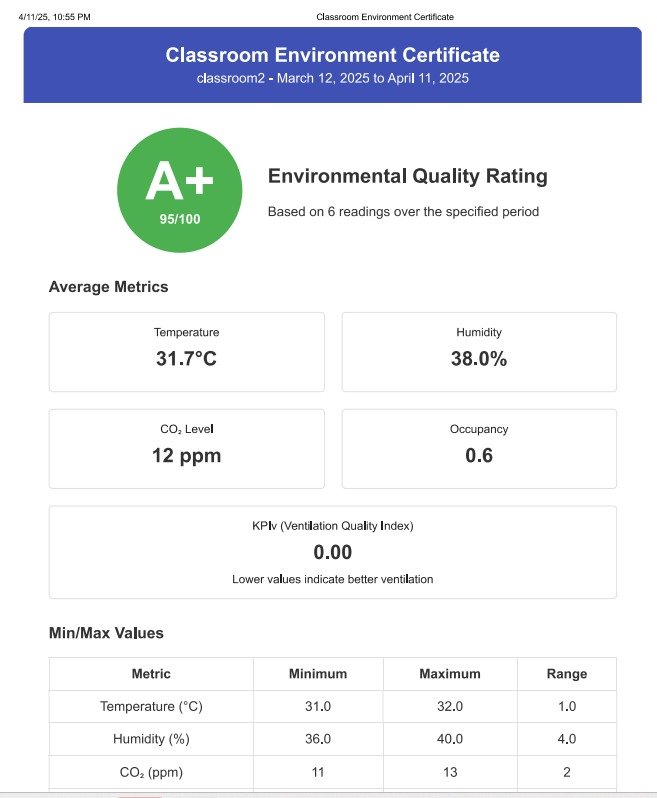
\includegraphics[width=0.8\textwidth]{Chapters/image (4).png}
		\caption{Generated Classroom Environmental Quality Certificate Including KPIV Score}
\end{figure}



\clearpage
\chapter{Conclusion and Future scope}
\section{Conclusion}
This work assessed the performance of an edge-based CO2 and occupancy prediction system to enhance classroom ventilation via real-time sensing and predictive analysis. The implementation of an LSTM-based model on an Arduino-Raspberry Pi hardware interface provided effective environmental monitoring and proactive control of ventilation, validated through performance measures and real-world outcomes. The outcome illustrates the system's efficiency, with the LSTM model performing successful future CO2 levels from past environmental data, such as temperature, humidity, and occupany. The model had low values of error when tested, with the Mean Absolute Error (MAE) and Mean Squared Error (MSE) reflecting stable convergence and high reliability. The built-in Arduino logic for tracking occupancy and estimation of trends and KPIv calculations allowed dynamic alerts and control of ventilation based on environmental thresholds. The hardware and software integration of components allowed end-to-end system real-time operation, such as automated certificate issuance for air quality compliance. The real-world effect of the system is seen through its capacity to enhance indoor air quality and guide ventilation choices based on intelligent predictions instead of reactive measures.

This system bridges the gap between low-cost IoT deployment and smart building management, enabling proactive ventilation control and data-backed environmental certification. Its accurate CO₂ and occupancy predictions, combined with dynamic certificate generation, showcase the value of custom hybrid models in complex, resource-constrained settings.
This system has the potential to serve as a foundational framework for smart educational infrastructure, sustainable indoor environments, and public health monitoring. By making ventilation assessment and control both accessible and intelligent, it supports the global movement toward healthier, data-informed, and energy-conscious indoor spaces.

\newpage
\section{Future Scope}
There are several concrete next steps to make this system more practical, scalable, and intelligent. Currently, the two Raspberry Pis communicate via a wired serial connection, which limits flexibility and real-world deployment. A major upgrade would be shifting to wireless communication using Zigbee, allowing better scalability and less physical constraint.

The machine learning model also needs improvement—training it on a larger, more diverse dataset will help increase accuracy and robustness. Moreover, scaling up the system to include more Raspberry Pis across different classrooms or zones can help validate the model’s generalizability and handle broader deployments.

On the hardware side, the project currently controls a basic fan to demonstrate actuator response. A realistic future direction is to interface with actual HVAC systems, enabling full integration into existing building infrastructure and making the system useful in real-world ventilation management.

In terms of environmental sensing, we could expand the scope by including sensors for PM2.5, VOCs, temperature, and humidity to create a more complete picture of indoor air quality. This data can improve model inputs and make the KPIv certification more meaningful.

Lastly, we aim to move toward real-time automation and intelligent adaptation—potentially using methods like federated learning for edge privacy and adaptive learning to fine-tune the system on the fly. Integration with Building Management Systems (BMS) could enable automatic HVAC adjustments based on predicted occupancy and air quality, leading to smarter, healthier, and more energy-efficient buildings.
\clearpage


% Appendix and Code Attachments

\fontsize{12pt}{12pt}\selectfont

\setstretch{1.0}
% Change Bibliography to References
\renewcommand\bibname{References}
\clearpage
\phantomsection
\addcontentsline{toc}{chapter}{References}
\printbibliography



%
% ---- Bibliography ----
%
% BibTeX users should specify bibliography style 'splncs04'.
% References will then be sorted and formatted in the correct style.
%
% \bibliographystyle{splncs04}
% \bibliography{mybibliography}
%
\begin{thebibliography}{00}
 \bibitem{1}
    Maohui Luo, Yumeng Hong, Jovan Pantelic (2021). Determining Building Natural Ventilation Potential via IoT-Based Air Quality Sensors. \textit{Frontiers in Environmental Science}, 9:634570. 
    
    \bibitem{2}
    Rastogi K, Lohani D, Acharya D (2021). Context-Aware Monitoring and Control of Ventilation Rate in Indoor Environments Using Internet of Things. \textit{IEEE Internet of Things Journal}, 8(11):9257–9267. 
    
    \bibitem{3}
    Mobasshir Mahbub, M. Mofazzal Hossain, Md. Shamrat Apu Gazi (2021). Cloud-Enabled IoT-based embedded system and software for intelligent indoor lighting, ventilation, early stage fire detection and prevention. \textit{Elsevier Publication}. 
    \bibitem{4}
    Lavinia Chiara Tagliabue, Fulvio Re Cecconi, Stefano Rinaldi, Angelo Luigi Camillo Ciribini (2021). Data driven indoor air quality prediction in educational facilities based on IoT network. \textit{Elsevier Publication}. 
     \bibitem{5}
    Jingyang Wang, Jiazheng Li, Xiaoxiao Wang, Jue Wang, Min Huang (2020). Air quality prediction using CT-LSTM. \textit{Springer}, Volume 33. 
    \bibitem{6}
    Guangfei Yang, Erbiao Yuan, Wenjun Wu (2021). Predicting the long-term CO2 concentration in classrooms based on the BO–EMD–LSTM model. \textit{Elsevier Publication}. 
     \bibitem{7}
    V. Faye McNeill, Richard Corsi, J. Alex Huffman, Cathleen King, Robert Klein, Michael Lamore, Do Young Maeng, Shelly L. Miller, Nga Lee Ng, Paula Olsiewski, Krystal J. Godri Pollitt, Rachel Segalman, Alex Sessions, Todd Squires, Sabrina Westgate (2022). Room-level ventilation in schools and universities. \textit{Elsevier Publication}. 
     \bibitem{8}
    S. Dhanalakshmi, M. Poongothai, Kaner Sharma (2020). IoT Based Indoor Air Quality and Smart Energy Management for HVAC System. \textit{Elsevier Publication}. 
    
 \bibitem{9}
    Rafael Fayos-Jordan, Jaume Segura-Garcia, Antonio Soriano-Asensi, Santiago Felici-Castell, Jose M Felisi, Jose M Alcaraz-Calero (2021). VentQsys: Low-cost open IoT system for \( CO_2 \) monitoring in classrooms. \textit{Springer}. 

     \bibitem{10}
     Rizzo; Camilleri; Gatt; Yousif(2024). Optimising Mechanical Ventilation for Indoor Air Quality and Thermal Comfort in a Mediterranean School Building. \textit{MDPI}. 
    
    \bibitem{11}
    Zivelonghi; Giuseppi, (2023). Smart Healthy Schools: An IoT-enabled concept for multi-room dynamic air quality control. \textit{Elsevier Publication}. 
     \bibitem{12}
        Zeba Idrees, Zhuo Zou, Lirong Zheng (2018). Edge Computing Based IoT Architecture for Low Cost Air Pollution Monitoring Systems: A Comprehensive System Analysis, Design Considerations \& Development. \textit{MDPI}. 
     \bibitem{13}
        Gonçalo Marques, Cristina Roque Ferreira, Rui Pitarma (2018). A System Based on the Internet of Things for Real-Time Particle Monitoring in Buildings. \textit{MDPI}. 
\bibitem{14}
    Hesham El-Sayed, Sharmi Sankar, Mukesh Prasad, Deepak Puthal, Akshansh Gupta, Manoranjan Mohanty (2017). Edge of Things: The Big Picture on the Integration of Edge, IoT and the Cloud in a Distributed Computing Environment. \textit{IEEE Access}. 
    \bibitem{15}
    Jagriti Saini, Maitreyee Dutta, Gonçalo Marques (2020). Indoor Air Quality Monitoring Systems Based on Internet of Things: A Systematic Review. \textit{MDPI}. 
    \bibitem{16}
    Mohieddine Benammar, Abderrazak Abdaoui, Sabbir H.M. Ahmad, Farid Touati, Abdullah Kadri (2018). A Modular IoT Platform for Real-Time Indoor Air Quality Monitoring. \textit{MDPI}. 
    \bibitem{17}
    Jung-Yoon Kim, Chao-Hsien Chu, Sang-Moon Shin (2014). ISSAQ: An Integrated Sensing Systems for Real-Time Indoor Air Quality Monitoring. \textit{IEEE Sensors Journal}. 
    \bibitem{18}
    Mehmet Ta¸stan and Hayrettin Gökozan (2019). Real-Time Monitoring of Indoor Air Quality with Internet of Things-Based E-Nose.\textit{MDPI}. 
    \bibitem{19}
    Kenichi Azumaa, Naoki Kagib, U. Yanagic, Haruki Osawad(2018). Effects of low-level inhalation exposure to carbon dioxide in indoor environments: A short review on human health and psychomotor performance.\textit{MDPI}
    \bibitem{20}
    Xilei Dai ,Wenzhe Shang ,Junjie Liu ,Min Xue ,Congcong Wang (2023) Achieving better indoor air quality with IoT systems for future buildings: Opportunities and challenges.\textit{MDPI}

    \bibitem{21}
    J. Chen, Y. Li, H. Wu, Y. Li, Z. Xu (2022). Transfer learning for cross-city air quality prediction. \textit{Elsevier Publication}
    \bibitem{22}
    S. Wu, Y. Li, Y. Wang, Y. Zhang, Y. Zhang (2022). Transfer learning-based detection of patient–ventilator asynchrony using pretrained convolutional neural networks. \textit{Elsevier Publication}

    \bibitem{23}
    Y. Wang, X. Li, J. Zhang, H. Wang, M. Huang (2023). Edge-adaptive CO2 prediction for indoor air quality using dynamic mobile window on IoT devices. \textit{Elsevier Publication}

    \bibitem{24}
    Zhang, Y. Liu, C. Wang, J. Liu, X. Dai (2021). IoT-based LSTM model for steady-state CO2 forecasting in smart buildings. \textit{Springer Publication}

    \bibitem{25}
    L. Sun, J. Wang, R. Chen, X. Liu, Y. Zhang (2022). IoT-driven model predictive control for real-time indoor ventilation and CO2 optimization on edge devices. \textit{IEEE Access.}
    \end{thebibliography}
    

\end{document}

